\documentclass[a4paper,titlepage]{report}

%PACKAGES
\usepackage[utf8]{inputenc}
\usepackage[T1]{fontenc}
\usepackage[francais]{babel}
\usepackage{amsmath}
\usepackage{amssymb}
\usepackage{mathrsfs}
\usepackage{fancyhdr}
\usepackage{lmodern}
\usepackage{graphicx}
\usepackage{geometry}
\usepackage{fancybox}
\usepackage{textcomp}
\usepackage{subfigure}
\usepackage{breqn}
\usepackage{color}
%Symbole euro
\usepackage{eurosym}

%Listings : affichage code
\usepackage{listings}

% Initialisation de listings
\definecolor{mymauve}{rgb}{0.63,0.13,0.94}
\definecolor{mygreen}{rgb}{0.13,0.55,0.13}
\definecolor{mybeige}{rgb}{0.99,0.99,0.86}
\definecolor{mygris}{rgb}{0.8,0.8,0.8}
\lstset{
    columns=flexible,
	numbers = left,				 	% placement de la numérotation des lignes
	numberstyle = \small,        	% taille du numéro de ligne
	stepnumber = 1,              	% ???
	numbersep = 10pt,            	% taille de l'espace de séparation entre numéro de ligne et code
	showspaces = false,          	% montrer les espaces
	showstringspaces=false,         % enlever les espaces str
	showtabs = false,            	% montrer les tabulations
	tab = rightarrowfill,        	% ???
	language = Matlab,             	% langage utilisé
	basicstyle = \small,			% ???
	captionpos = b,					% ???
	linewidth=\linewidth,			% largeur de la fenetre de code
	breaklines = true,				% ???
	commentstyle = \color{mygreen}\usefont{T1}{pcr}{m}{sl}, % définition de la couleur des commentaires
	stringstyle = \color{mymauve},  % définition de la couleur des chaines de caracteres
	identifierstyle = \ttfamily,    % ???
	keywordstyle = \color{blue},	% définition de la couleur des mots clés
	frame=single,
	backgroundcolor=\color{mybeige},
}



%Elements de la page de garde
\begin{document}

\begin{titlepage}

\begin{figure}
\centering

\includegraphics[width=5cm]{logo-ulg.png}
\end{figure}



\title{
\vspace{0.2cm}
\LARGE{\textbf{Projet 1 - Chaînes de Markov}} \\ \textsc{Eléments de processus stochastiques}
\author{\textbf{Floriane Magera} \\ \textbf{Romain Mormont} \\ \textbf{Fabrice Servais}\\ Troisième bachelier en sciences de l'ingénieur}
\date{}
\rule{15cm}{1.5pt}
}

%\geometry{hmargin=2.5cm}
\end{titlepage}

%DOCUMENT
\pagestyle{fancy}
\lhead{Projet 1 - Chaînes de Markov}
\rhead{Éléments de processus stochastiques}

%Page de garde
\maketitle
\newpage
\tableofcontents
\newpage
\chapter{Question 1}
\section{Etude du modèle de base}
\paragraph{2)} Avant de calculer la matrice de transition, il est nécessaire de caractériser la marche aléatoire. Autrement dit, il faut définir les poids/probabilités que nous appliquerons aux arêtes du graphe sur lequel le surfeur va évoluer. Nous avons déduit de l'énoncé du projet que les différentes possibilités de quitter un nœud devaient être \textbf{équiprobables} et nous utiliserons donc cette hypothèse dans la suite du rapport.
\paragraph{}
Suite à ce choix, la formation de la matrice de transition est très simple. Si l'on note $A$ la matrice d'adjacence, alors il suffit d'appliquer la formule suivante pour calculer l'élément Q(i,j) :
\[
Q(i,j) = A(i,j) \times \frac{1}{n}\sum\limits_{j = 1}^n A(i,j)
\]
Cette formule permet de placer à $0$ les éléments de $Q$ représentant une transition impossible et de placer à une certaine probabilité les autres éléments de $Q$ (toute probabilité non nulle d'une ligne de Q étant équiprobable comme attendu).
\paragraph{3)} Nous avons choisi un nombre de pas $t = 20$. Le cas où le surfeur démarre aléatoirement sur le graphe est représenté par une distribution initiale $\pi_0$ uniforme et le cas où il démarre d'une page fixe est représenté par une distribution initiale $\pi_0$ où toutes les probabilités sont nulles sauf celle située l'index correspondant au nœud de départ. L'évolution des probabilités dans les deux cas est donnée sur le Figure \ref{fig:q113}.
\begin{figure}[h]
	\center
	\subfigure{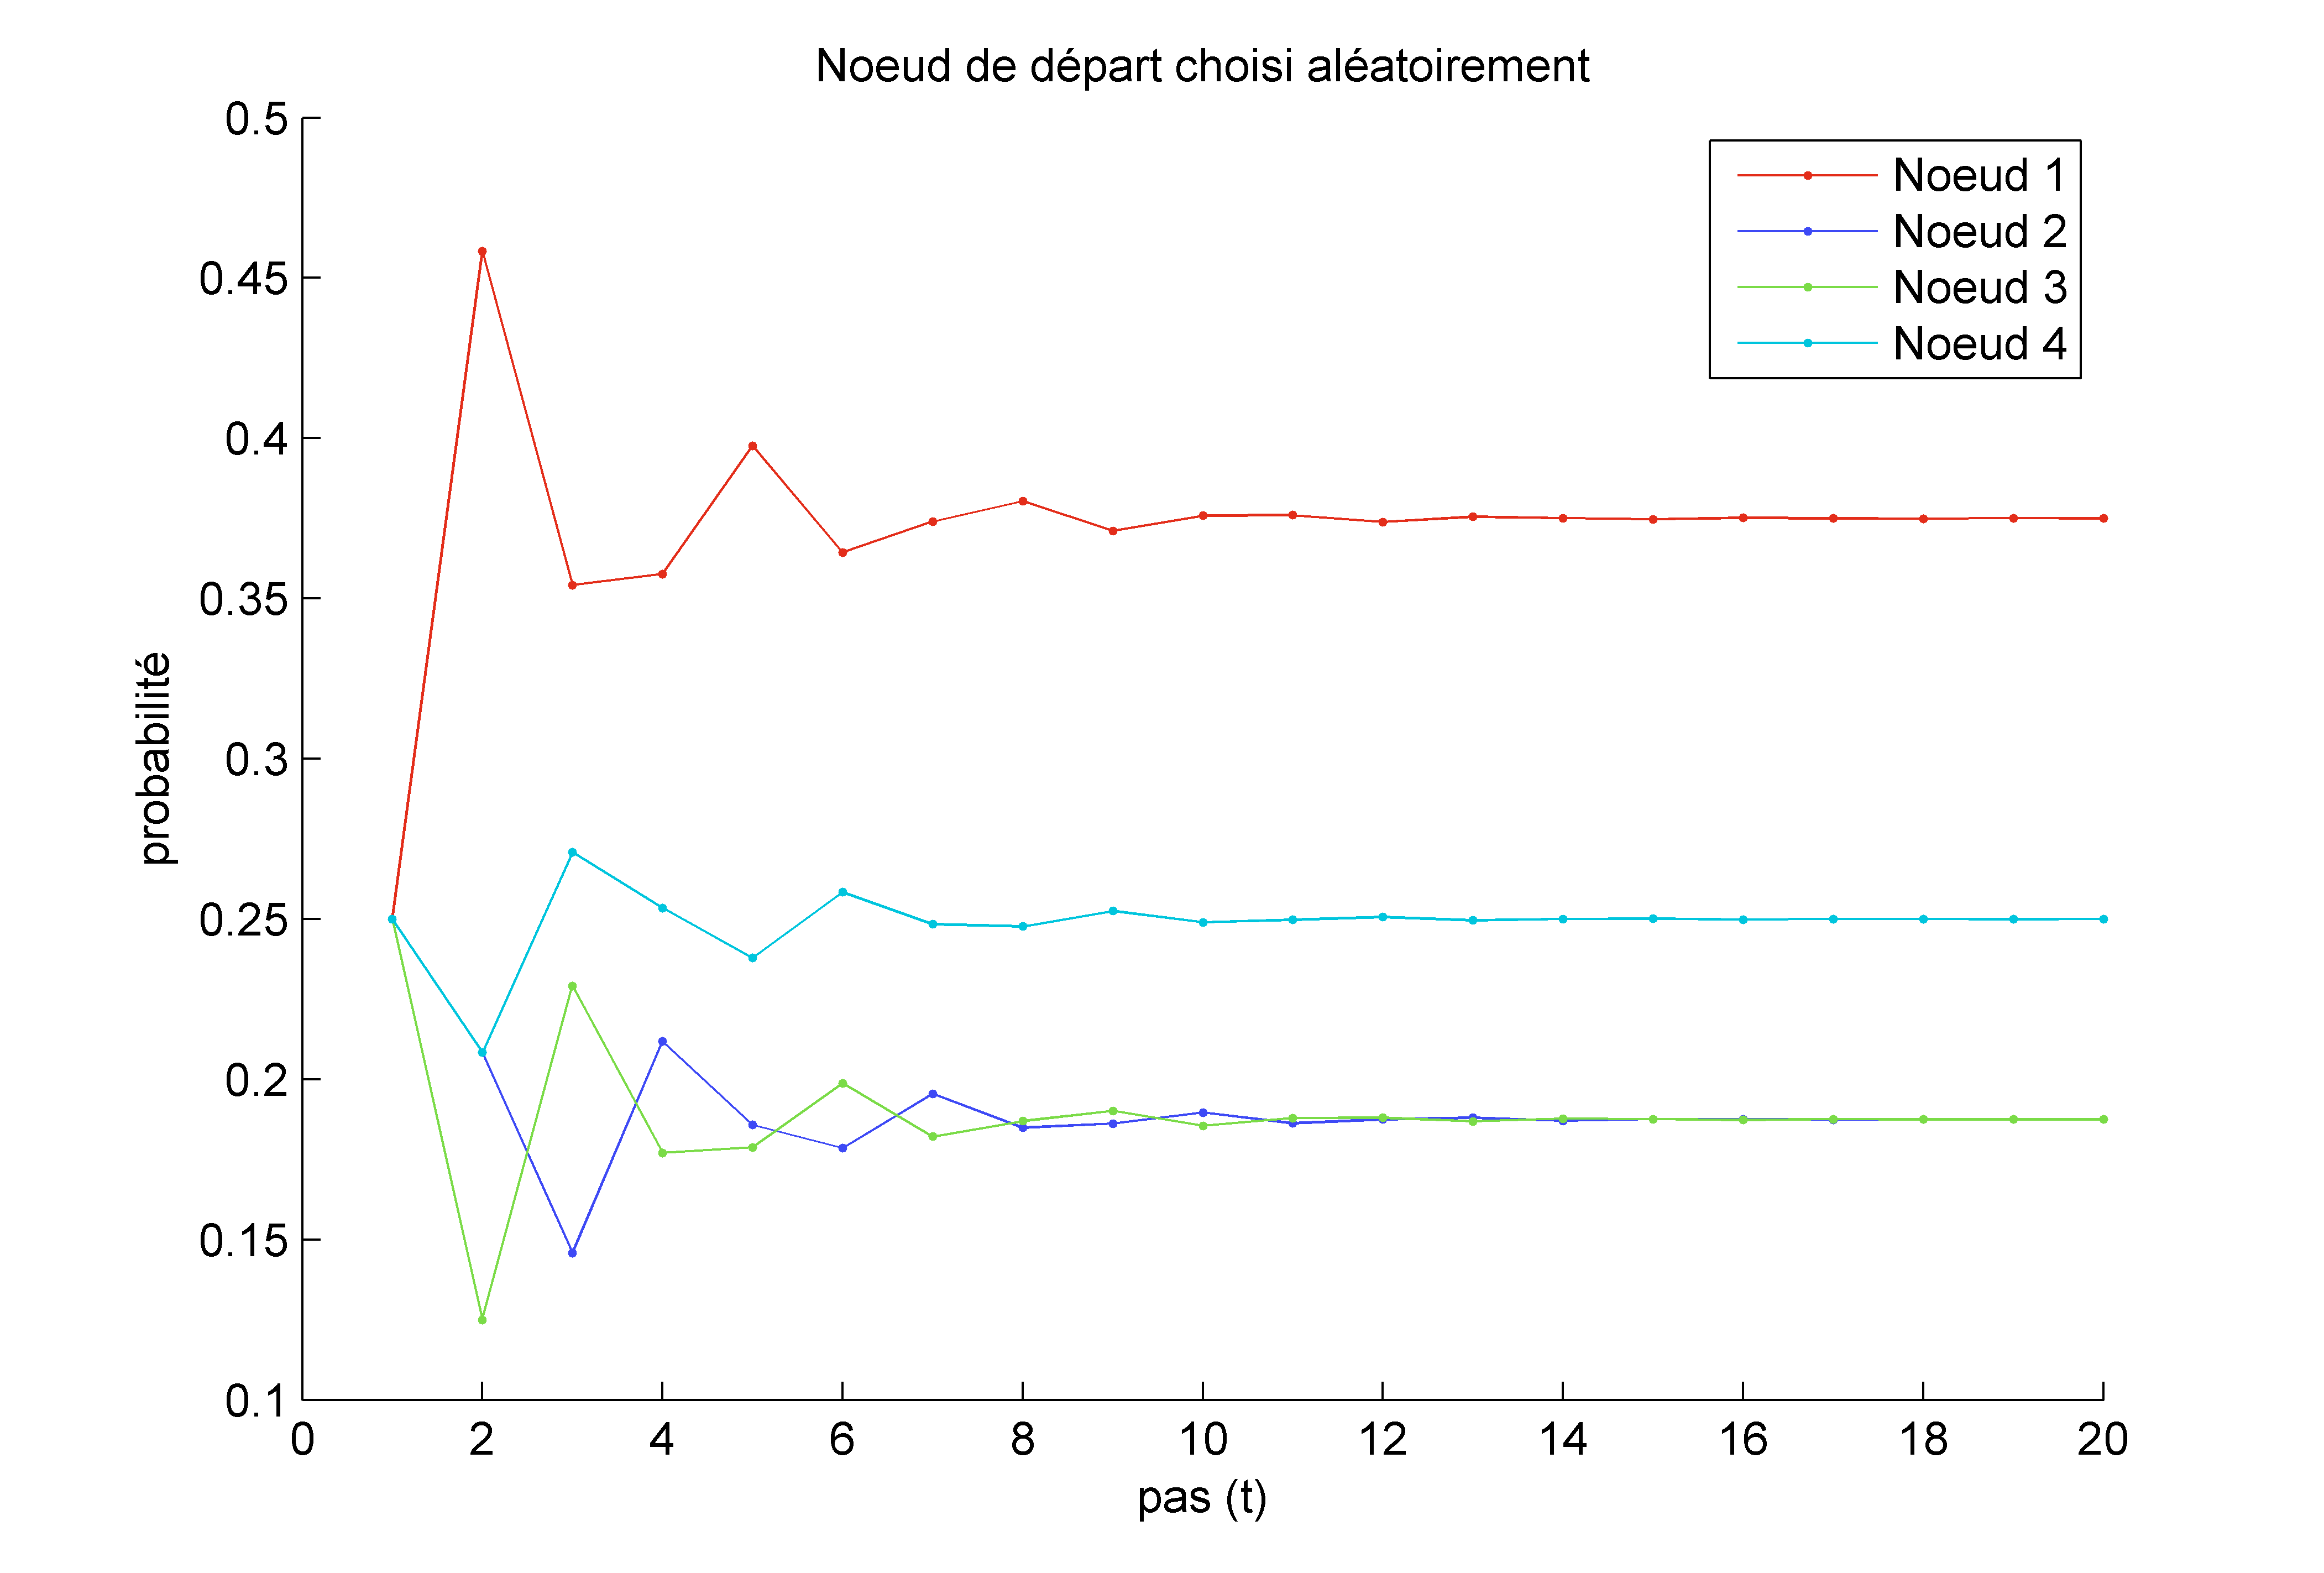
\includegraphics[scale=0.35]{../images/q1131_proba.png}}
	\subfigure{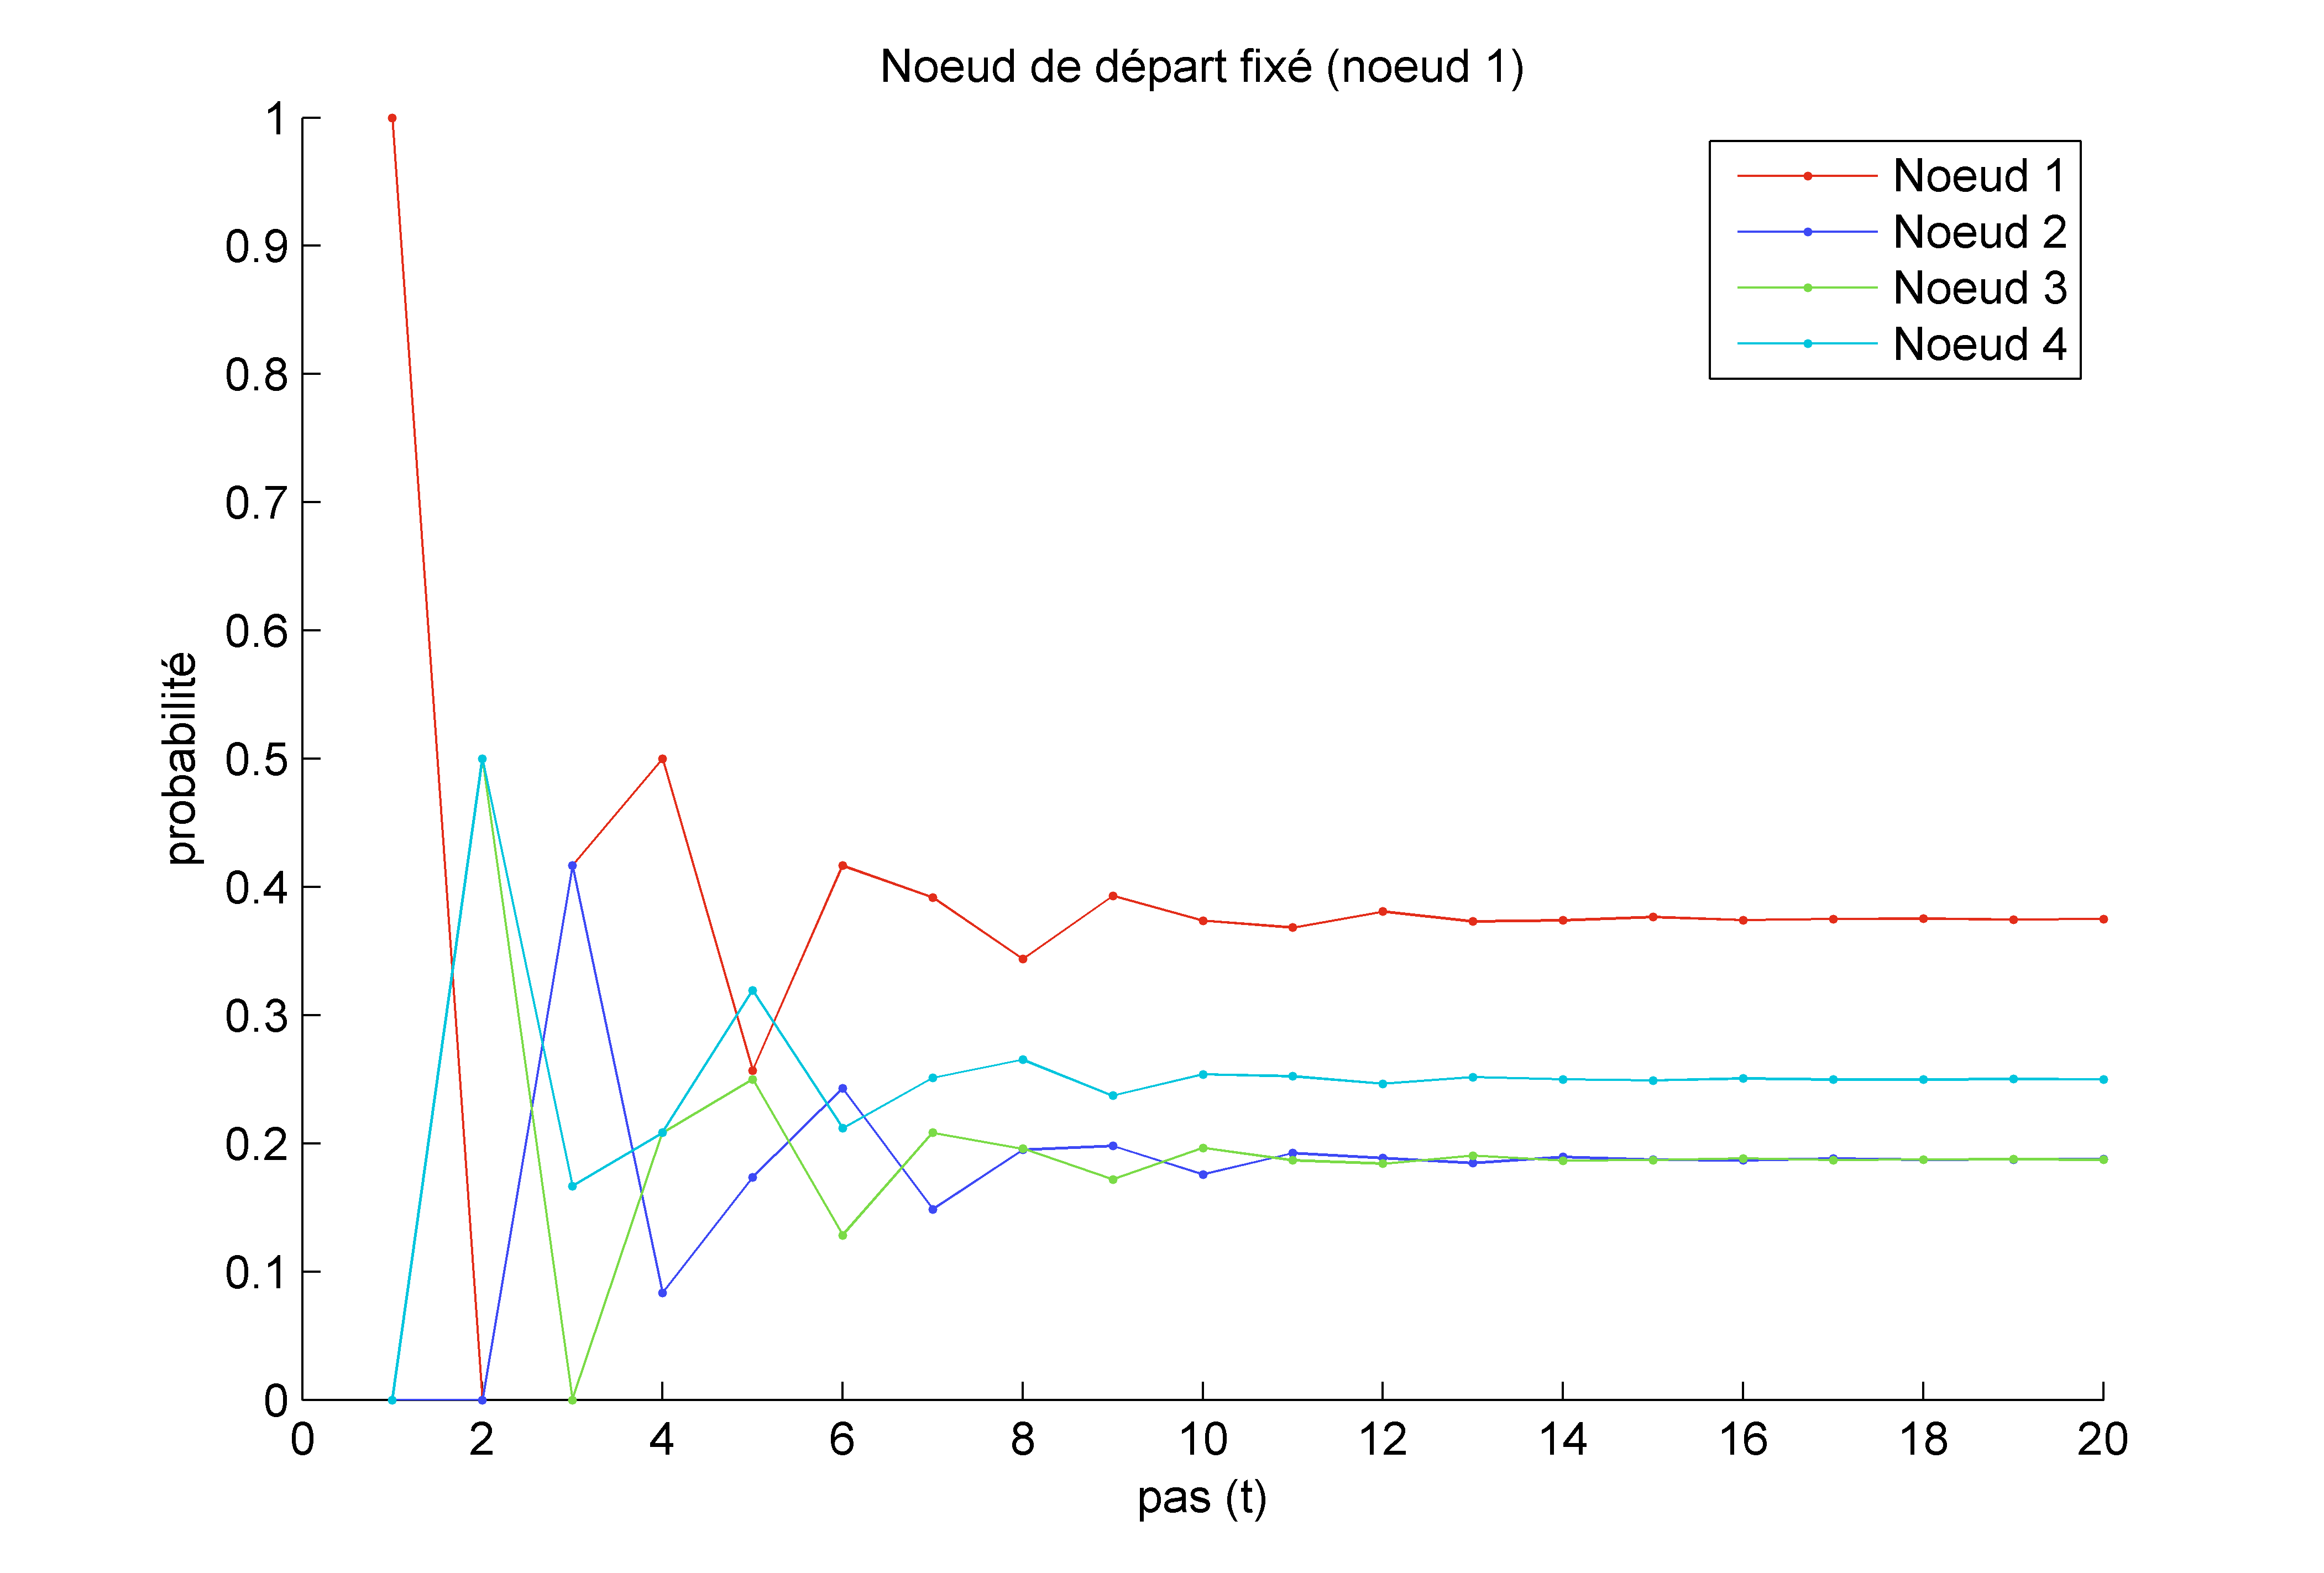
\includegraphics[scale=0.35]{../images/q1132_proba.png}}
	\caption{Évolution de la distribution de probabilité}
	\label{fig:q113}
\end{figure}
\paragraph{}
La matrice $Q^{(20)}$ obtenue est la suivante :
\[
Q^{(20)} = 
\begin{pmatrix}
 0.3751 & 0.1874 & 0.1875 & 0.2500\\
 0.3751 & 0.1877 & 0.1874 & 0.2499\\
 0.3749 & 0.1875 & 0.1875 & 0.2500\\
 0.3749 & 0.1875 & 0.1875 & 0.2500\\
\end{pmatrix}
\]
Si on observe les matrices $Q^{(k)}$ pour $k> 20$, on peut constater que les éléments se stabilisent et que les lignes s'égalisent. 
\paragraph{4)} La distribution stationnaire a été calculée par la méthode des puissances. Nous avons donc multiplié les distributions $\pi^{(k)}$ successives par $Q$ jusqu'à ce que cette distribution ce stabilise. Le critère de stabilisation choisi était le suivant : 
\[
\max\left(\left|\pi_j^{(k)} - \pi_j^{(k - 1)}\pi\right|\right) < \varepsilon
\]
où $\pi_j$ est la $j^{\text{ième}}$ composante du vecteur $\pi$. La distribution stationnaire obtenue est donnée ci-dessous :
\[
\pi_\infty = 
\begin{pmatrix}
0.3750 &
0.1875 &
0.1875 &
0.2500 \\
\end{pmatrix}
\]
On constate que les lignes de la matrice sont très proches
\paragraph{5)} On constate que le noeud 1 possède le meilleur PageRank, suivi des noeuds 2 et 3 à égalité et du noeud 4. On peut expliquer ce classement intuitivement : 
\begin{itemize}
	\item le \textbf{noeud 1} possède le plus d'arêtes entrantes donc ayant le plus de chance d'être visité
	\item le \textbf{noeud 3} possède le moins d'arêtes entrantes donc ayant le moins de chance d'être visité
	\item les \textbf{noeuds 2} et \textbf{4} possèdent le même nombre intermédiaire (par rapport aux deux autres) d'arêtes entrantes. Le PageRank du noeud 4 est néanmoins plus élevé que celui du noeud 2 puisque le noeud 4 possèdent une arête entrante venant du noeud 1 qui est le plus visité.
	\item malgré un nombre d'arête entrante plus élevé que pour le noeud 3, le \textbf{noeud 2} possède une PageRank égal. Cela est dû au fait que, d'une part, le noeud 3 peut être visité depuis le noeud le plus visité (noeud 1) ce qui améliore son PageRank et, d'autre part, que le noeud 2 ne peut être accéder depuis des noeuds moins visités (noeud 3 et 4) ce qui abaisse son PageRank. 
\end{itemize} 
\paragraph{6)} Dans un premier temps, nous avons généré une chaîne pour chaque longueur. Le résultat obtenu est donné sur la Figure \ref{sfig:q116_evol_1}. On peut déjà observer que les différentes courbes obtenues oscillent autour de leur probabilité stationnaire correspondante. Néanmoins, étant donné la présence d'oscillations, nous avons décidé de refaire l'expérience en générant cette fois-ci 1000 chaînes pour chaque longueur. Nous avons ensuite moyenné les différentes probabilités afin d'obtenir un résultat plus précis (voir Figure \ref{sfig:q116_evol_2}). Les courbes obtenues nous permettent de confirmer les premières observations.
\paragraph{}
Remarquons aussi que, quelque soit la distribution de départ, la distribution converge vers la distribution stationnaire.
\begin{figure}[h]
	\center
	\subfigure[1 génération]{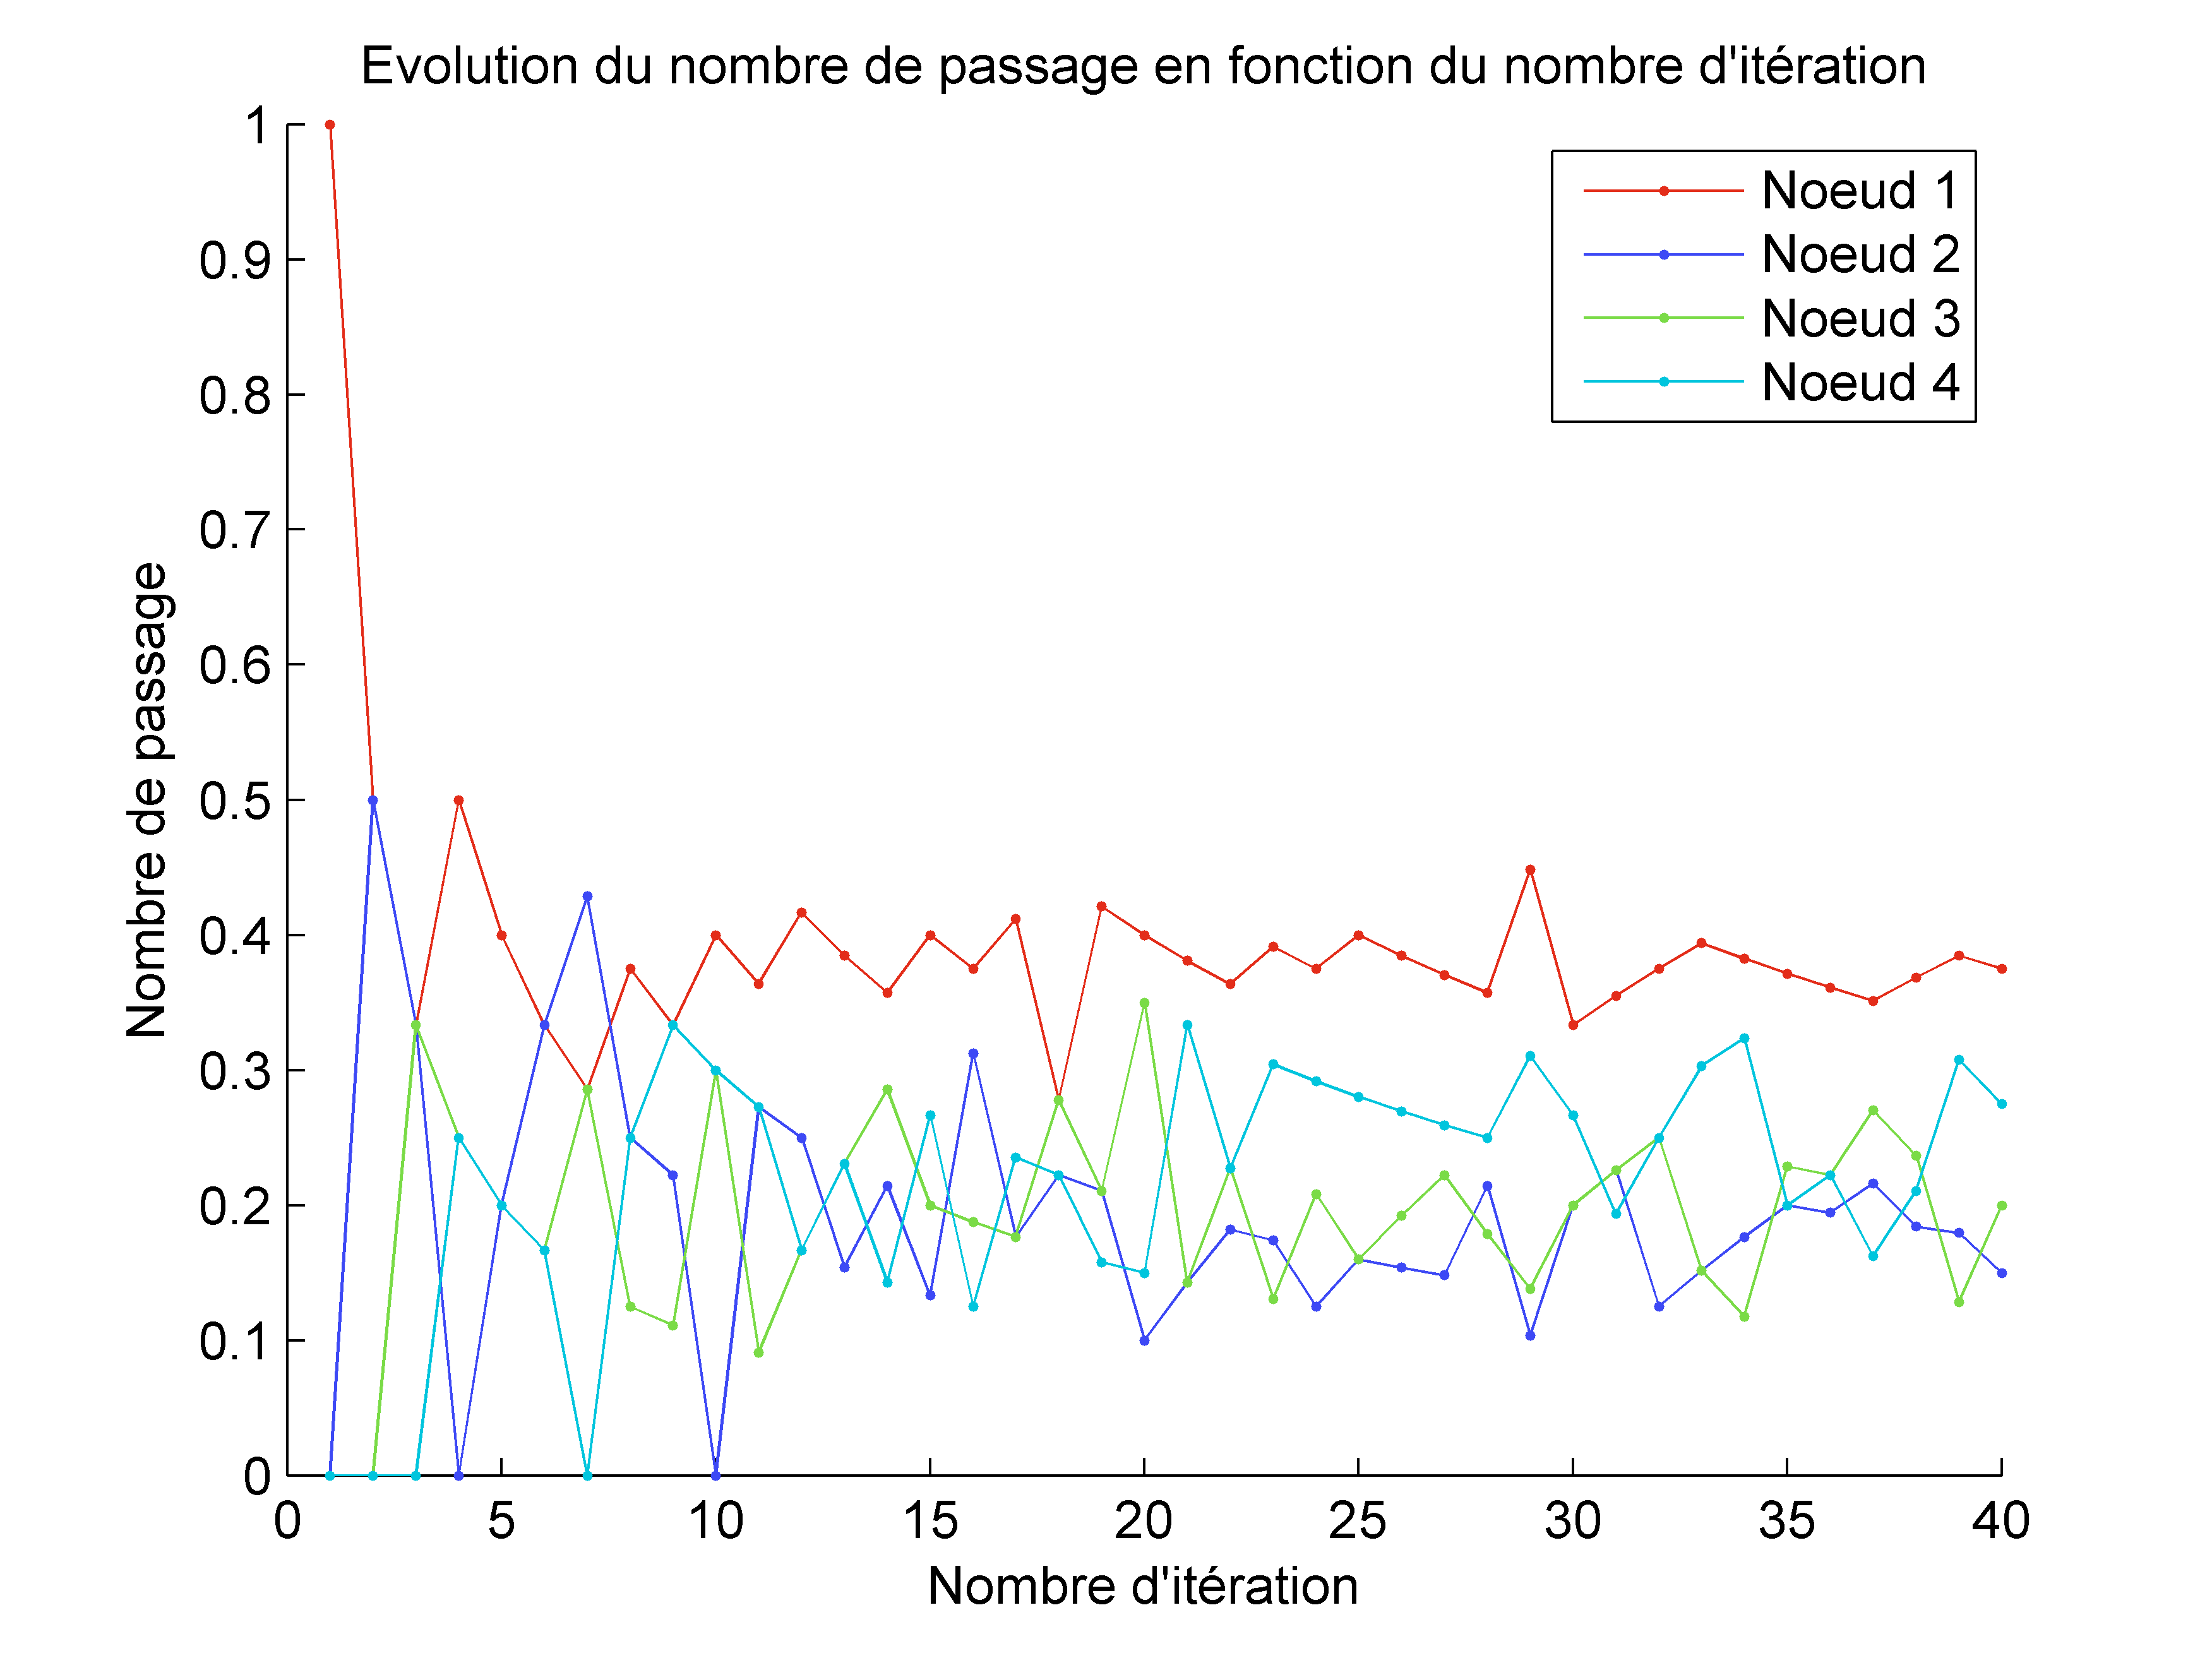
\includegraphics[scale=0.45]{../images/q116_evol_1.png}\label{sfig:q116_evol_1}}
	\subfigure[1000 générations]{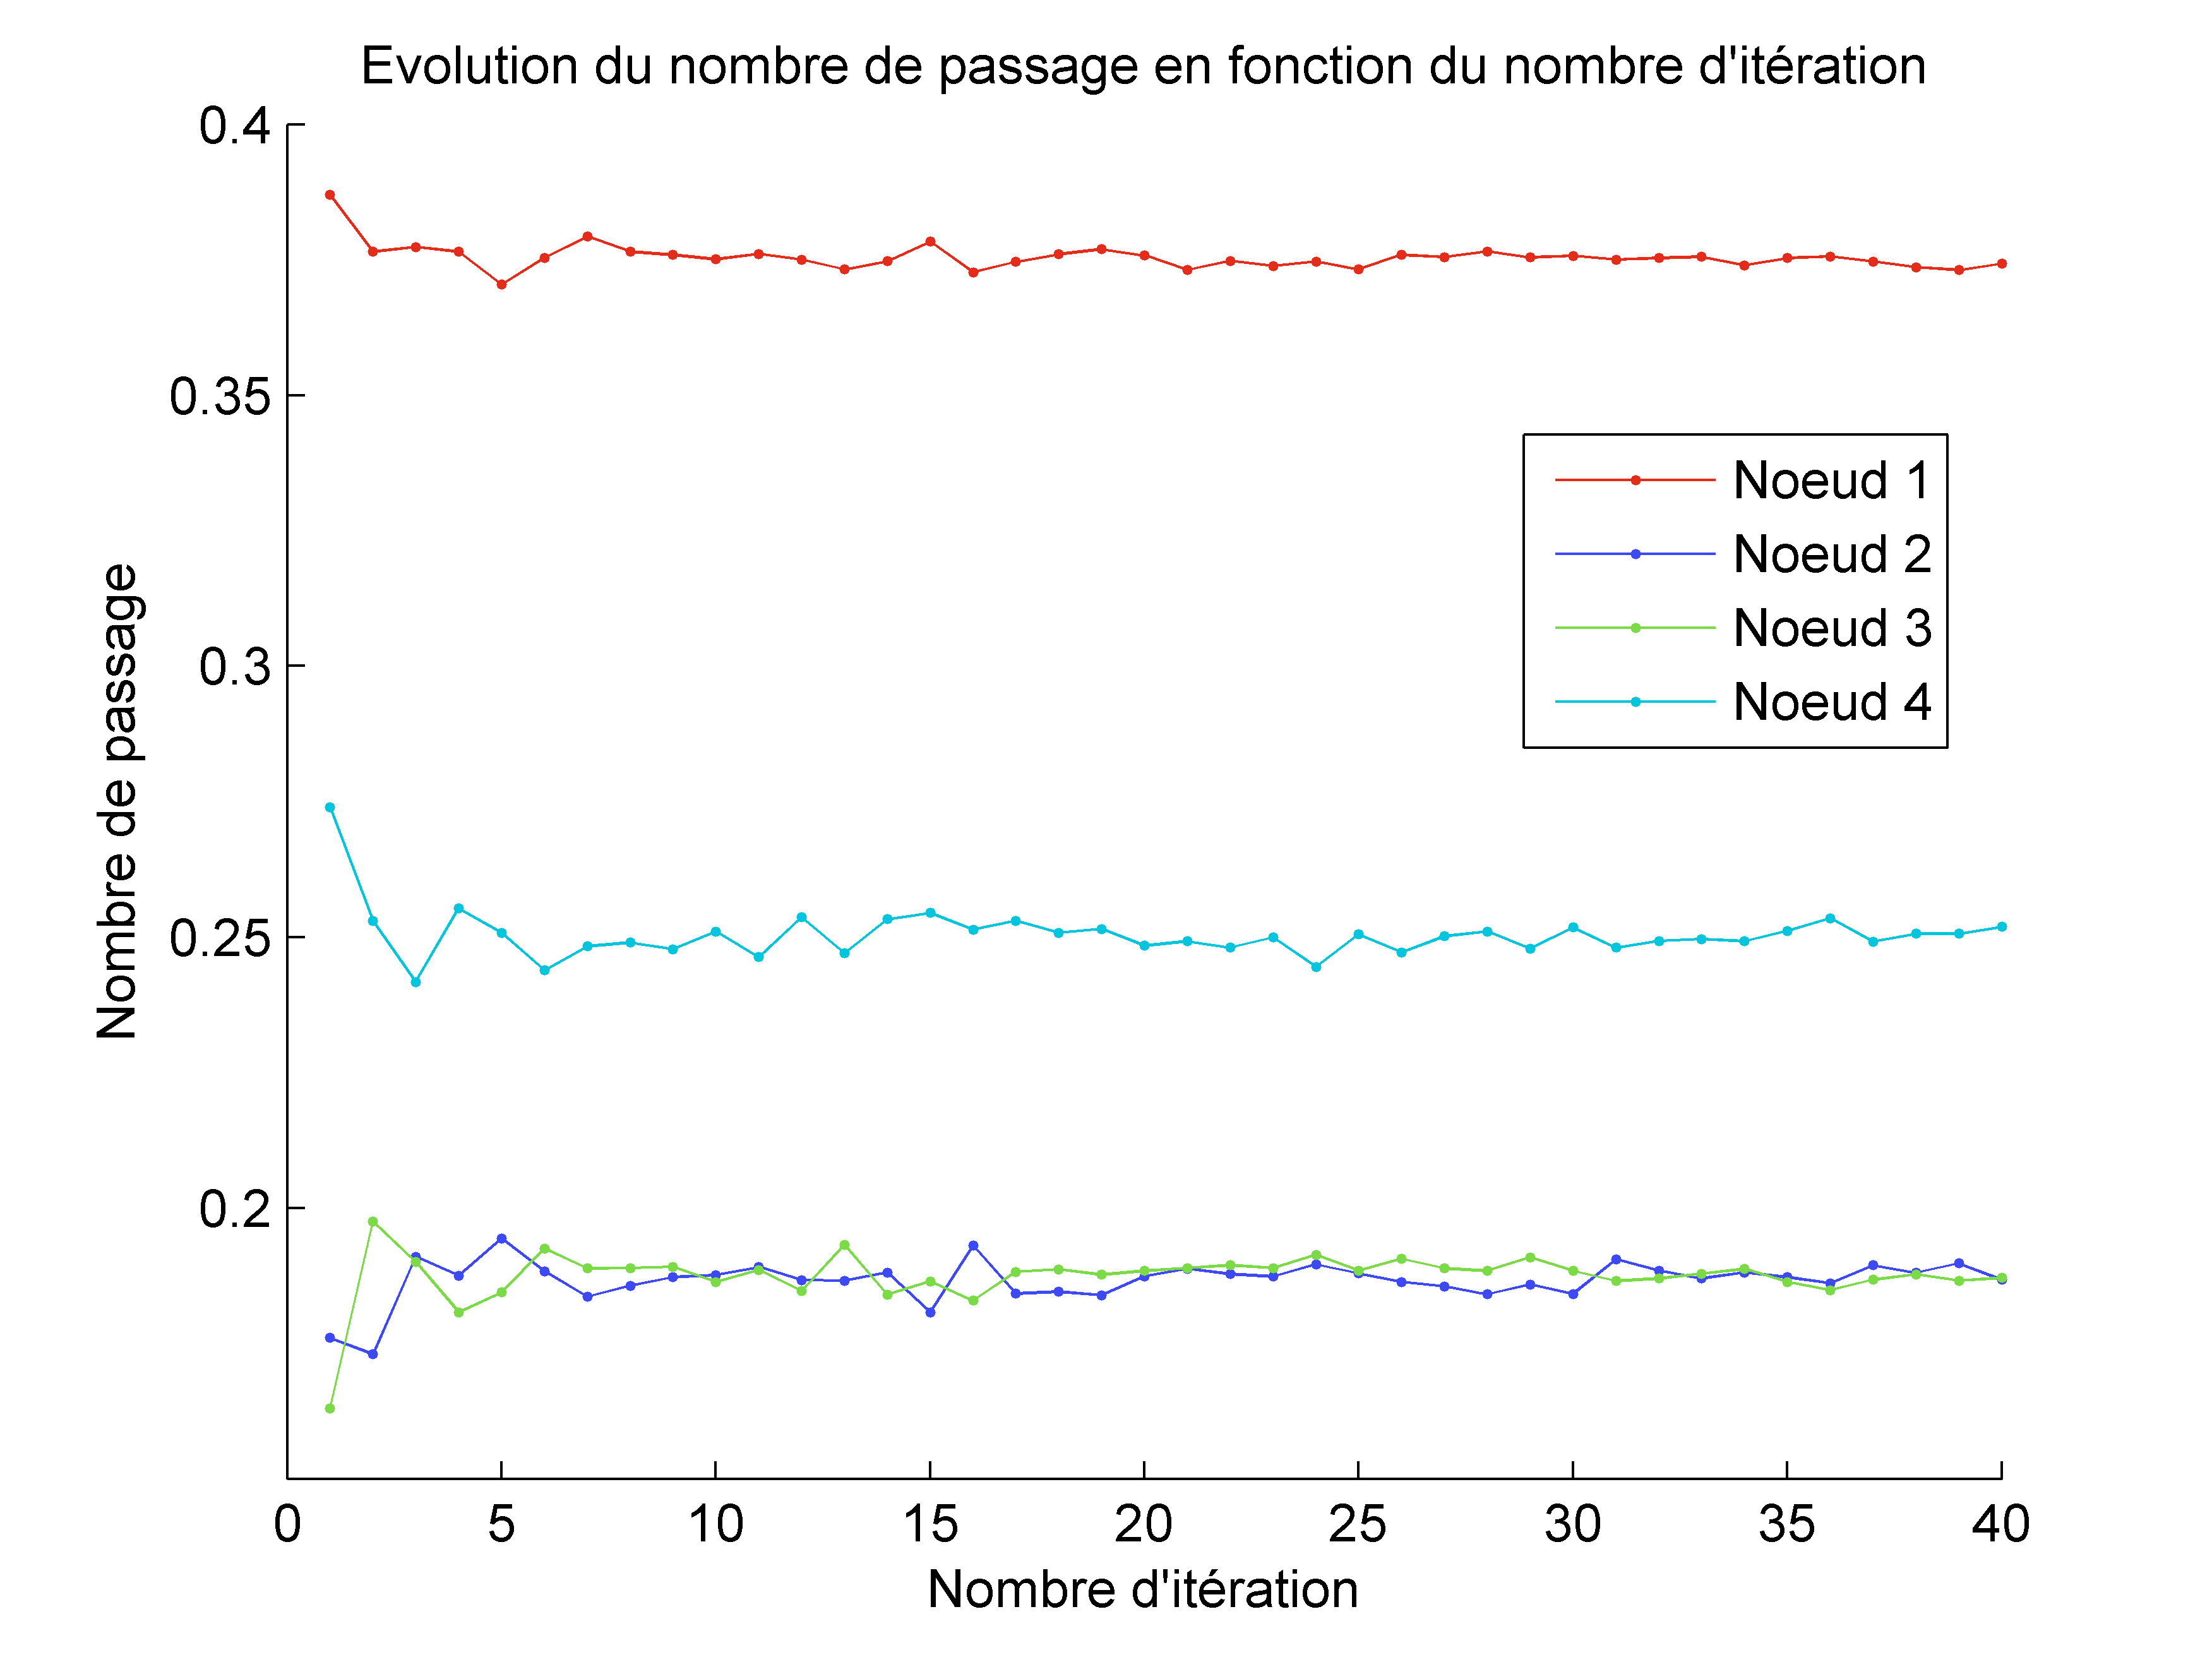
\includegraphics[scale=0.45]{../images/q116_evol_2.png}\label{sfig:q116_evol_2}}
	\caption{Évolution du nombre de passage par un noeud}
\end{figure}
\paragraph{7)} 
\subsection{Analyse des matrices $A_2$ et $A_3$}
\paragraph{1)} Pour pouvoir calculer des éventuelless distribution stationnaires sur base des matrices $A_2$ et $A_3$, nous avons calculés les matrices de transition $Q_2$ et $Q_3$ : 
\[
Q_2 = 
\begin{pmatrix}
         0 &   1.0000  &       0  &       0 \\
         0 &        0  &       0  &  1.0000 \\
    0.5000 &   0.5000  &       0  &       0 \\
    1.0000 &        0  &       0  &       0 \\
\end{pmatrix}
Q_3 = 
\begin{pmatrix}
        0  &   1.0000   &      0  &       0  &       0 \\
    1.0000 &        0   &      0  &       0  &       0 \\
         0 &   0.3333   &      0  &  0.3333  &  0.3333 \\
         0 &        0   &      0  &       0  &  1.0000 \\
         0 &        0   &      0  &  1.0000  &       0 \\
\end{pmatrix}
\]
Nous avons ensuite appliqué la méthode des puissance pour obtenir des distributions $\pi^{(k)}$ successives. Le résultat est donné sur la Figure \ref{fig:q118}. On constate qu'aucune distribution stationnaire n'a pu être trouvée étant donné la présence d'\textbf{oscillations}.
\paragraph{}
On constate aussi que la \textbf{probabilité} d'atteindre une certain nœud \textbf{tombe à 0} ou est directement nulle dès la première itération dans les deux situations. Ce phénomène est dû à la présence de \textit{dangling nodes} dans les deux graphes. On peut directement voir la présence de type de nœud sur les matrices de transitions :  elle se manifeste par une colonne composée uniquement de probabilités nulles et implique qu'il est impossible de passer d'un nœud quelconque au \textit{dangling node}.
\paragraph{}
Ces deux phénomènes sont précisément des \textbf{limitations} du modèle du surfeur aléatoire simpliste présenté dans cette première partie. D'une part, les oscillations empêchent d'atteindre une distribution stationnaire. D'autre part, la probabilité nulle d'atteindre un nœud existant rend l'éventuelle distribution stationnaire (et donc le PageRank) peut représentative de l'organisation des nœuds puisqu'elle en omet d'en prendre certains en compte.
\paragraph{}
Les\textbf{ causes de ces phénomènes} sont d'une part la présence d'un cycle  infini dans les graphes et la présence de \textit{dangling nodes}. Ces problèmes vont être contournés en introduisant la téléportation dans la section suivante.
\begin{figure}[h]
	\center
	\subfigure[Distribution initiale uniforme]{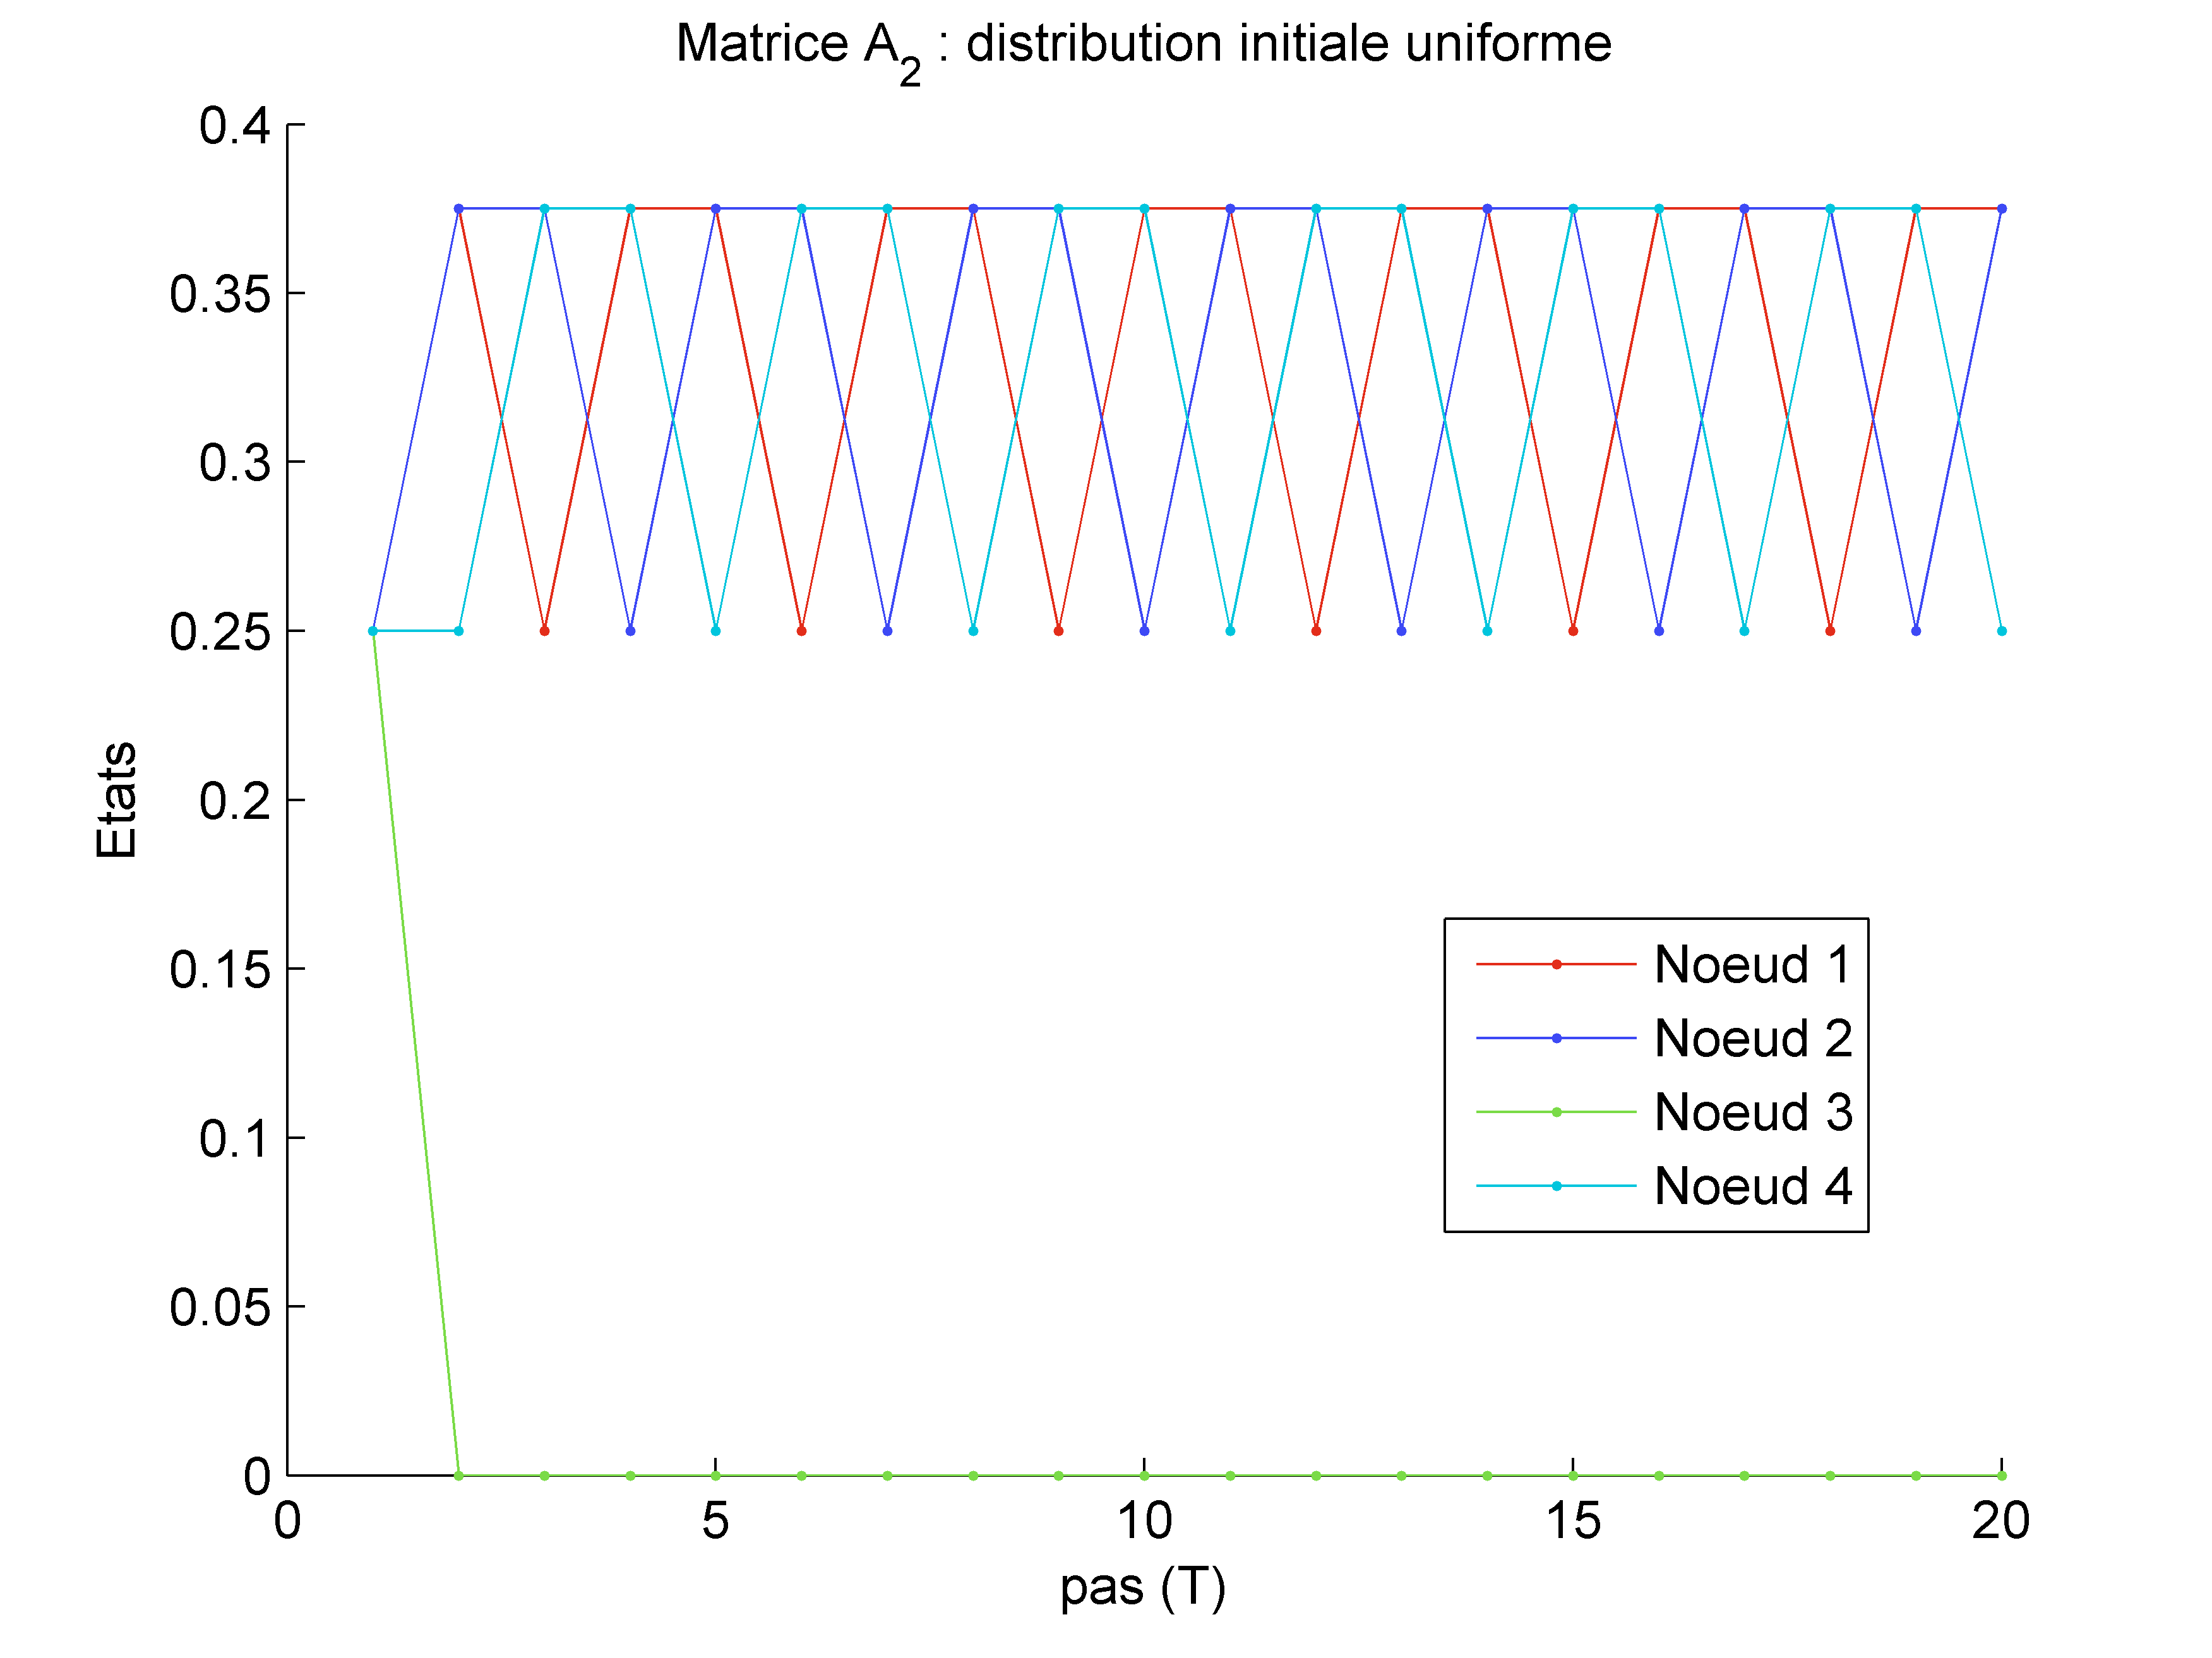
\includegraphics[scale=0.45]{../images/q118_evol_21.png}\label{sfig:q118_evol}}
	\subfigure[Depuis le noeud 1]{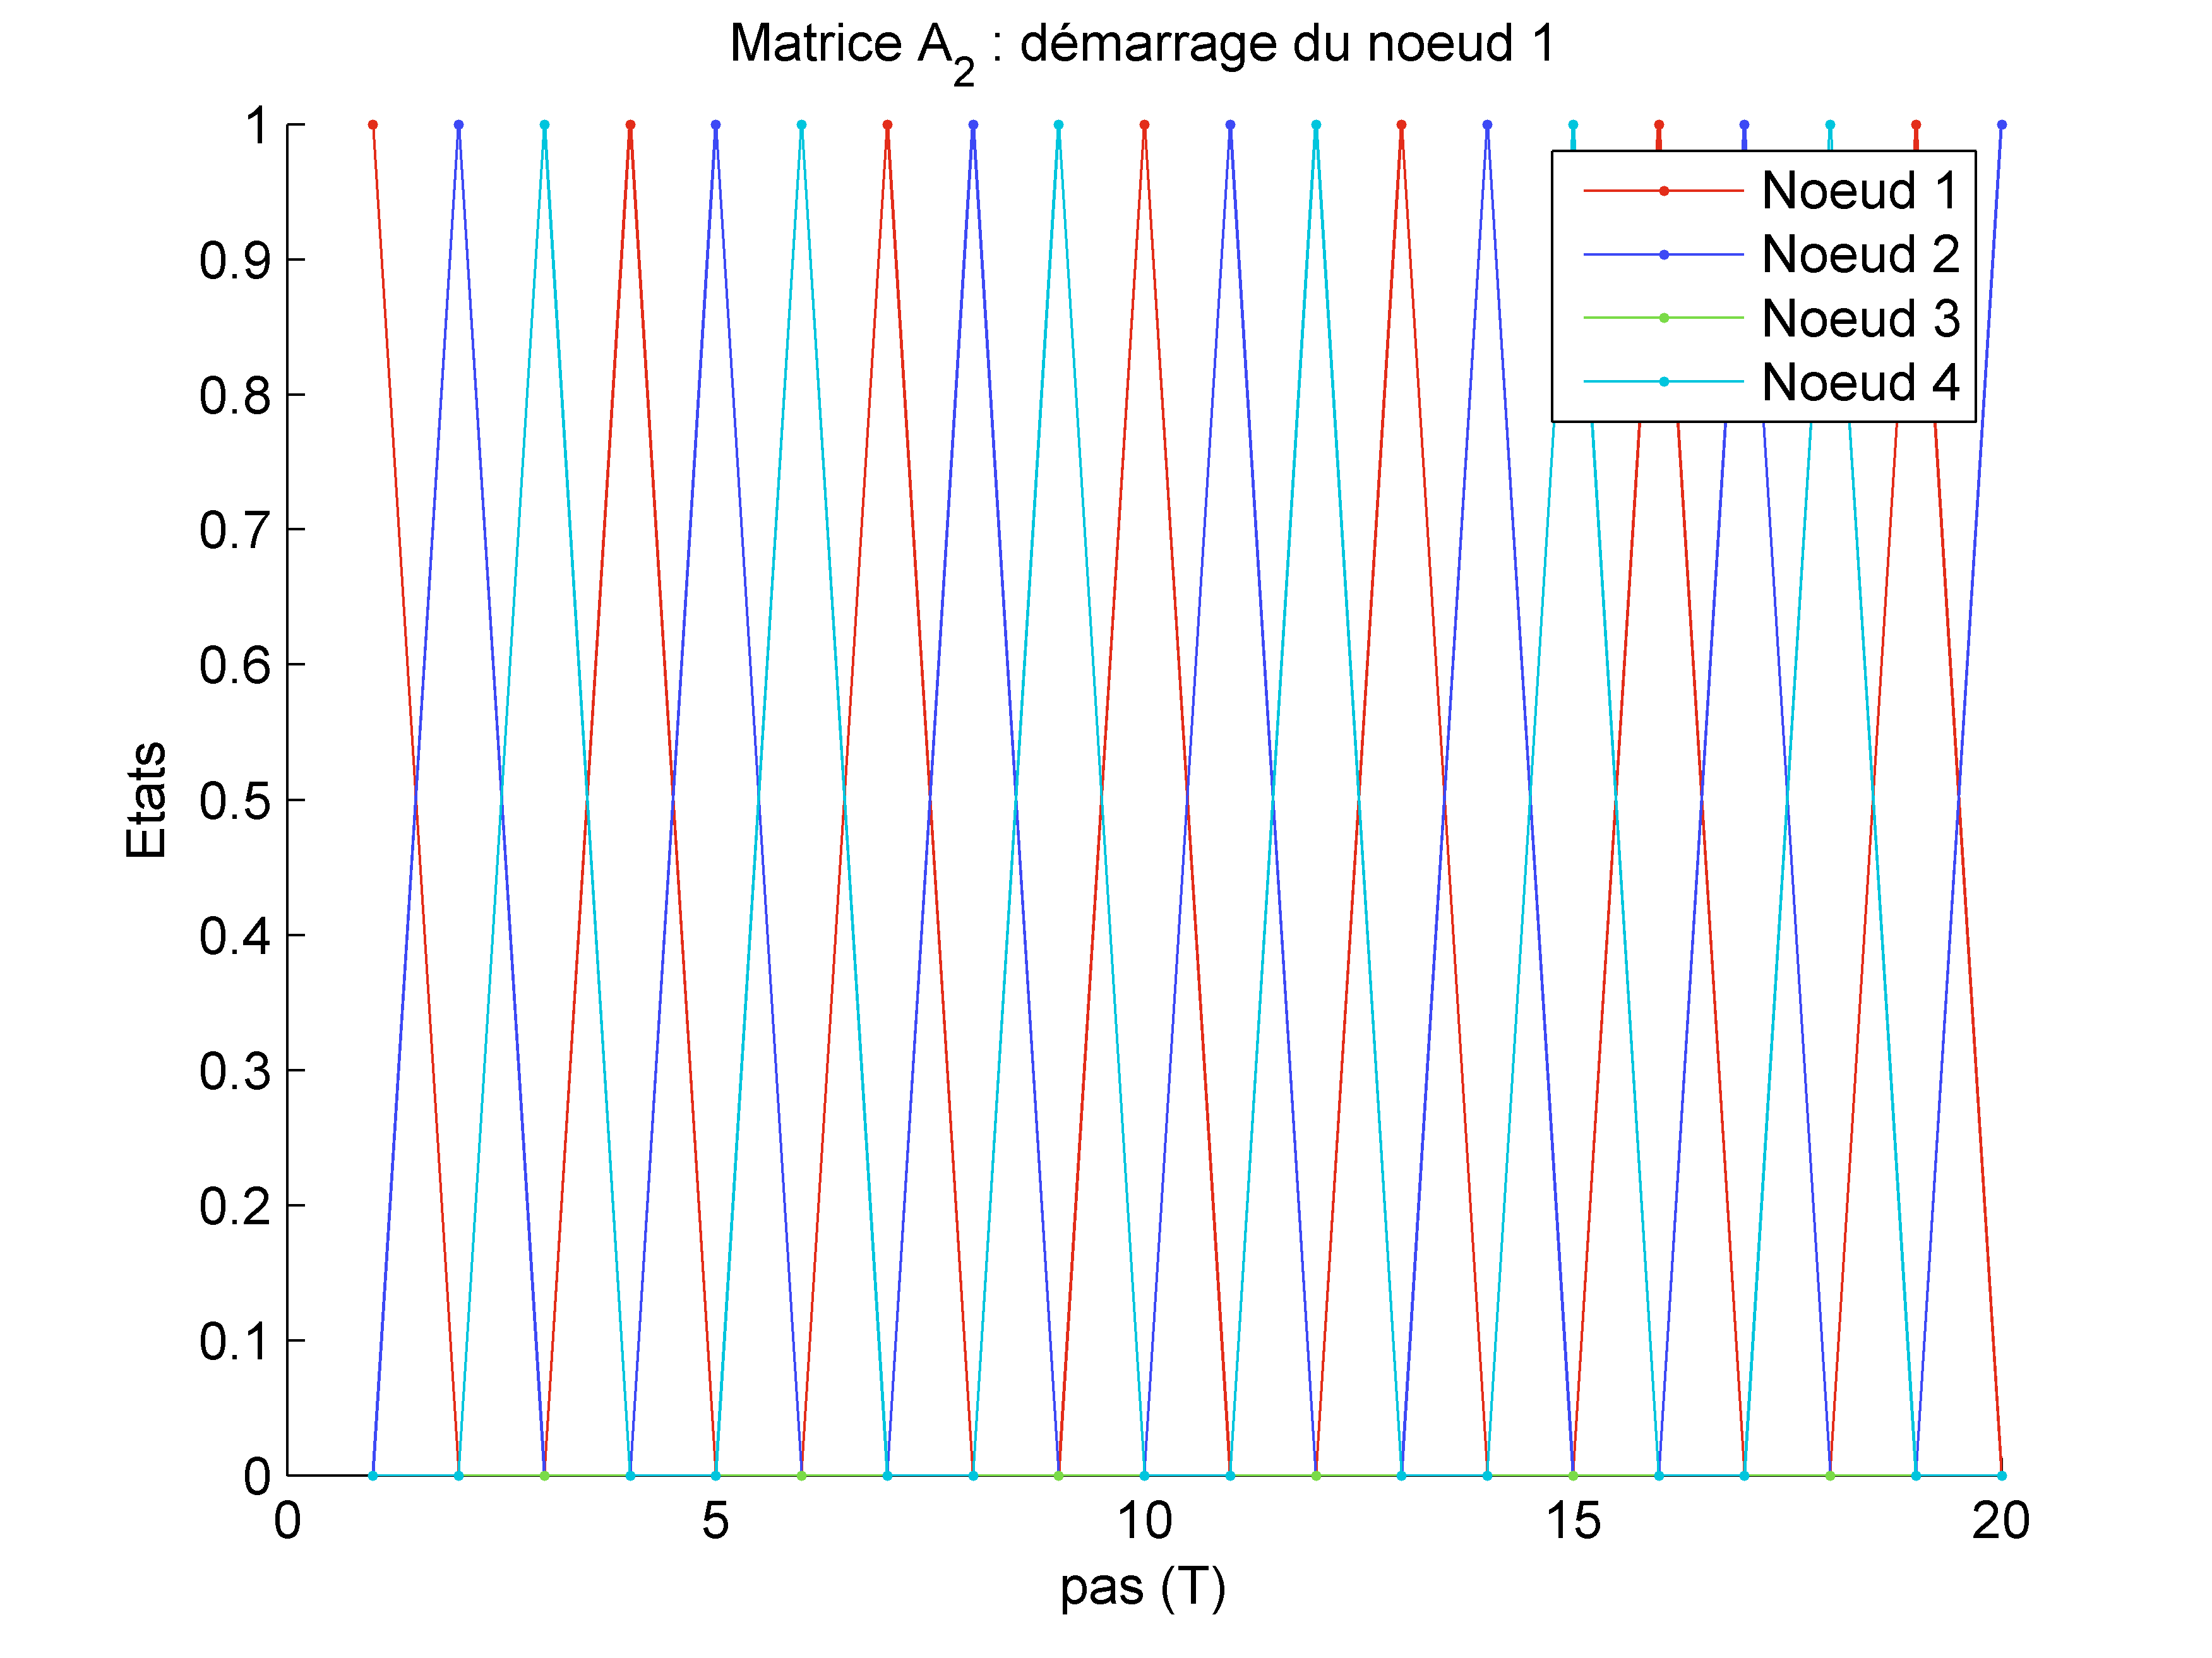
\includegraphics[scale=0.45]{../images/q118_evol_22.png}\label{sfig:q118_evol}}
	\subfigure[Distribution initiale uniforme]{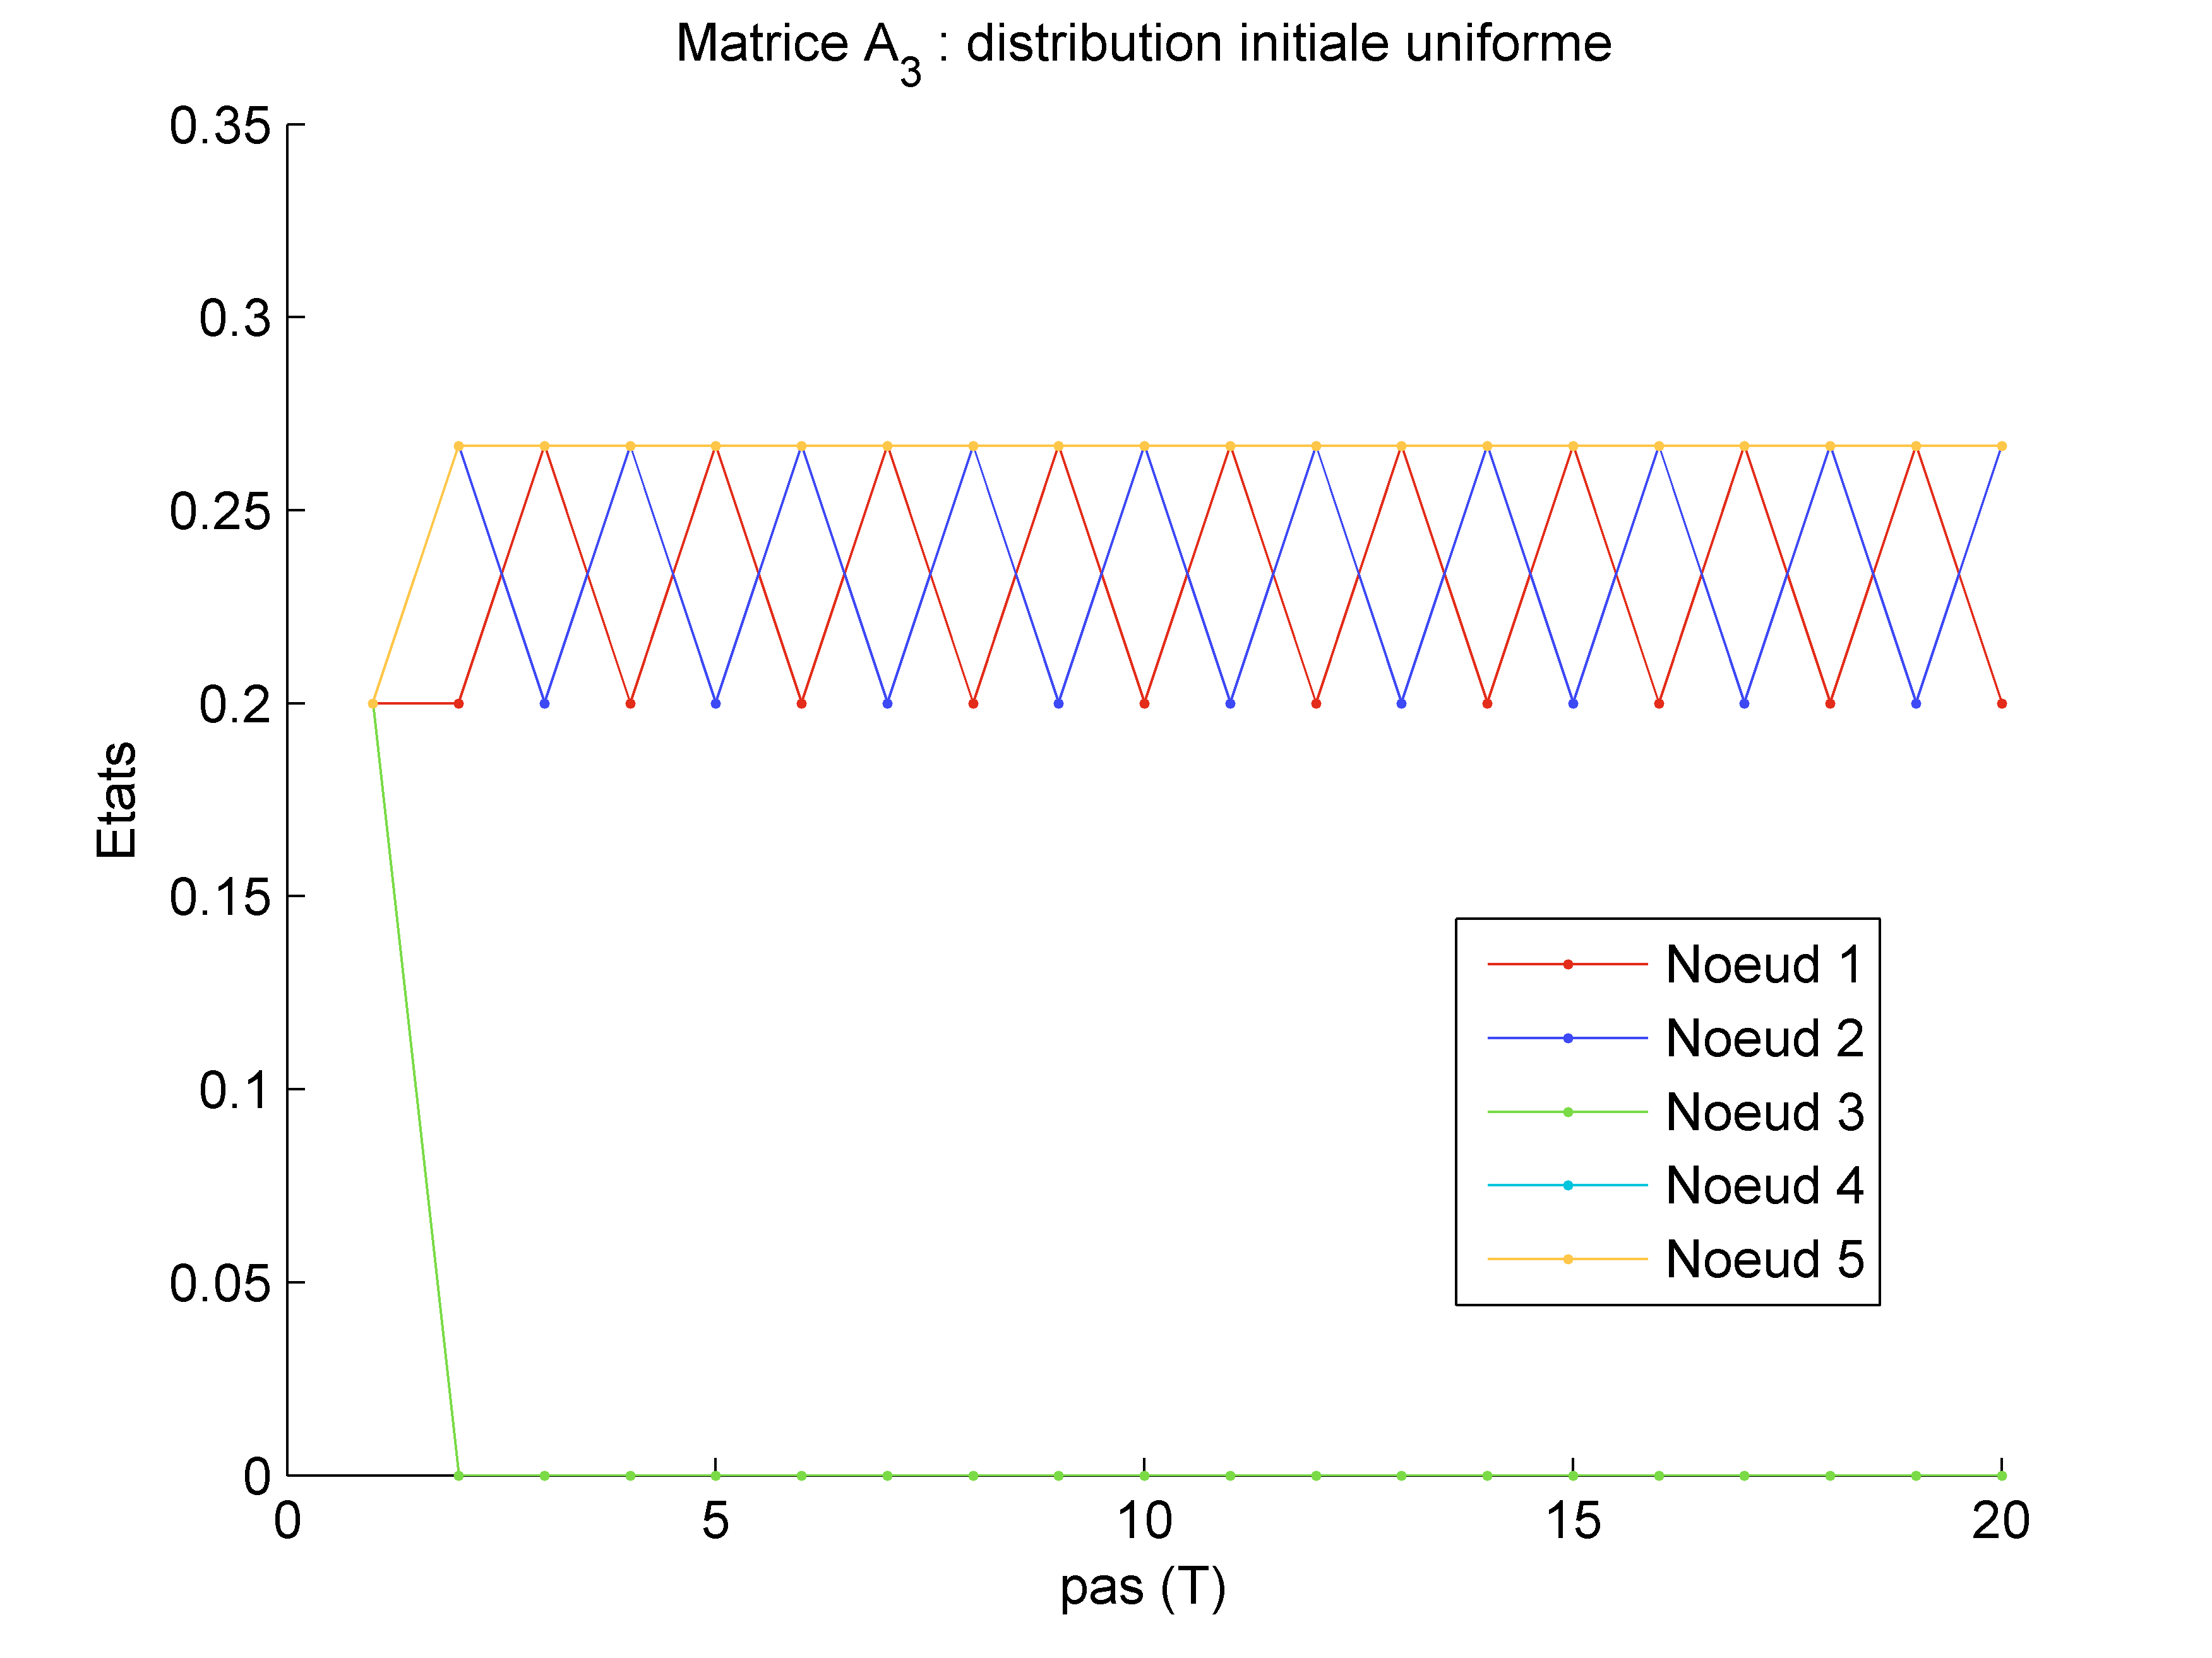
\includegraphics[scale=0.45]{../images/q118_evol_31.png}\label{sfig:q118_evol}}
	\subfigure[Depuis le noeud 1]{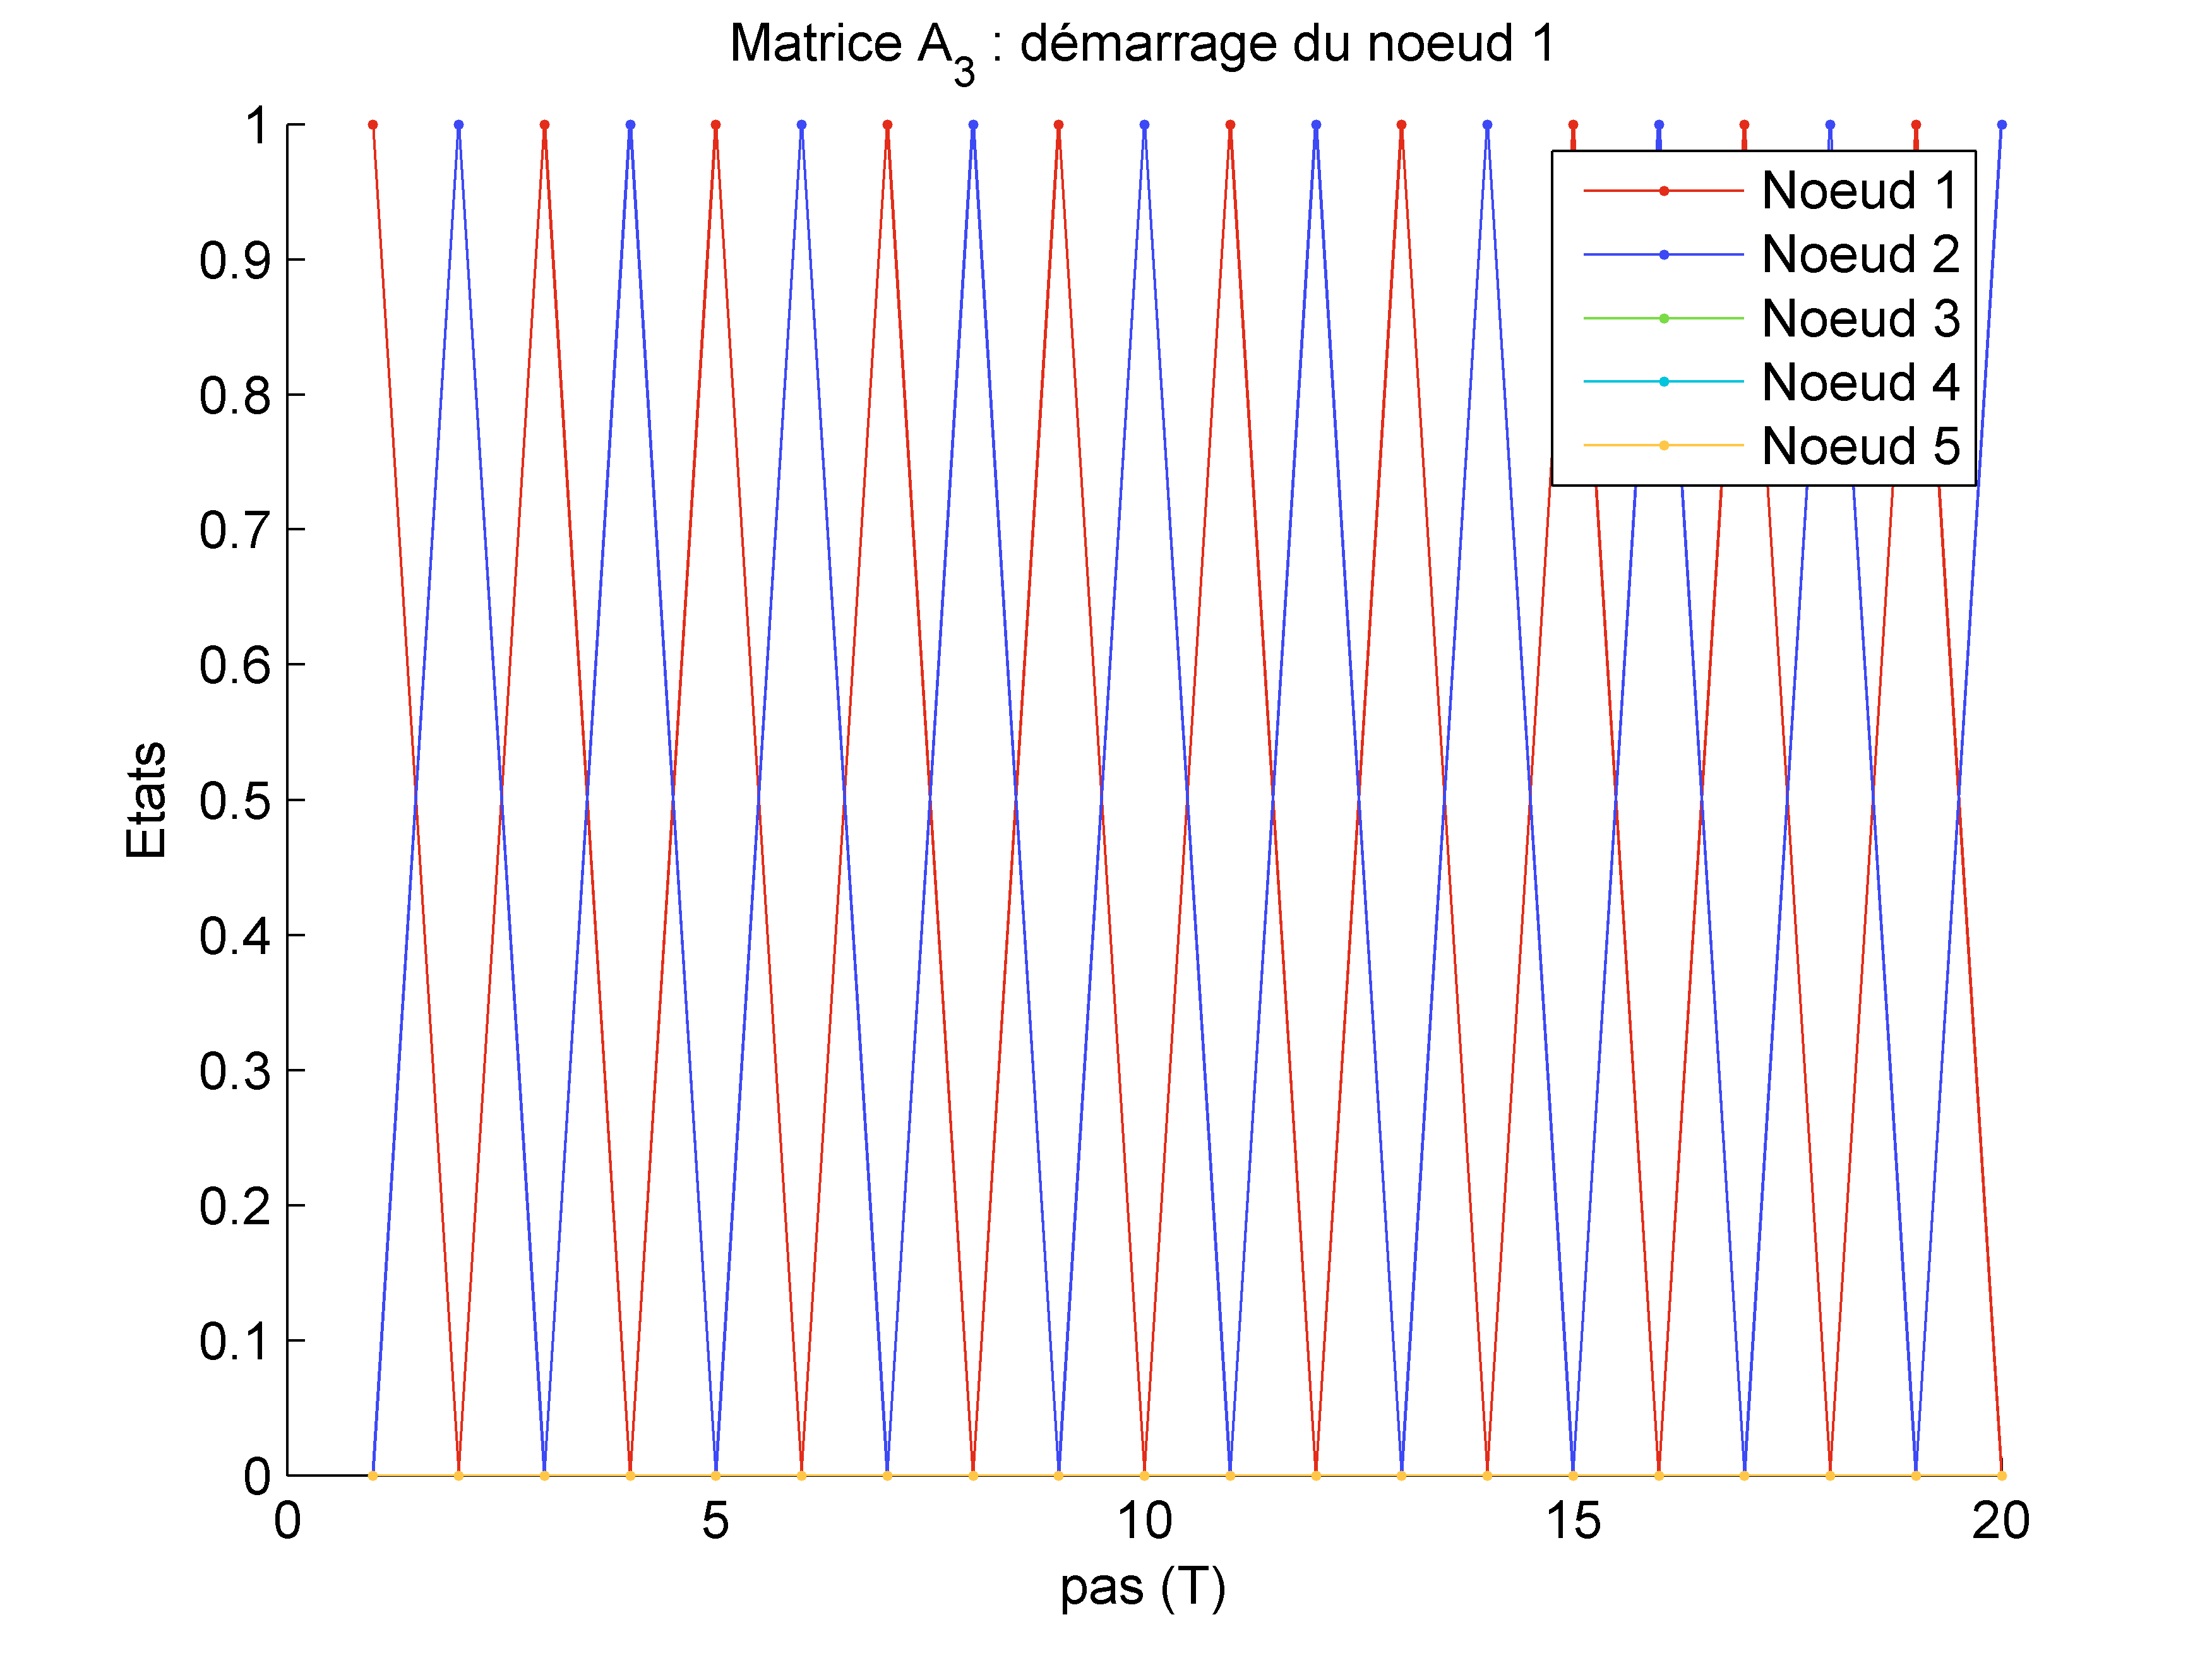
\includegraphics[scale=0.45]{../images/q118_evol_32.png}\label{sfig:q118_evol}}
	\caption{Évolution des distributions de probabilités}
	\label{fig:q118}
\end{figure}
\paragraph{2)} 
\section{Téléportation}
\paragraph{1)}
La formule utilisée pour calculer la matrice de transition $Q_t$ du modèle du surfeur avec téléportation est la suivante :
\[
	Q_t = (1 - \alpha) Q' + \alpha \tilde{Q}
\]
où $Q'$ et $\tilde{Q}$ sont des matrices de transition et $\alpha$ la probabilité de téléportation. 
\paragraph{}
La première est la matrice de transition du graphe initial auquel on a rajouté des arêtes partant des \textit{dangling nodes}. Elle a été calculée en remplaçant par $\frac{1}{n}$ tous les éléments de la matrice $Q$ situés dans des lignes ne contenant que des 0. Cette valeur $\frac{1}{n}$ a été choisie en considérant une densité de probabilité uniforme entre les différentes arêtes partant des \textit{dangling nodes}. 
\paragraph{}
La seconde est la matrice de transition du graphe complet formé des noeuds du graphe initial. Autrement dit, la matrice de transition représentant la téléportation. Une combinaison linéaire de paramètre $\alpha$ est ensuite appliquée aux deux matrices pour trouver la matrice $Q_t$.
\paragraph{2)}
Pour que la distribution stationnaire $\pi_s$ soit unique, \textbf{il faut que la chaîne de Markov soit irréductible}. Autrement dit, il faut que pour tout couple de nœuds $(i_1$, $i_2)$, il existe une arête les reliant (un probabilité non-nulle de passer de $i_1$ à $i_2$). Cette propriété est vérifiée avec le modèle du surfeur modifié puisque la téléportation permet, depuis tout noeud, de se diriger vers un autre noeud tant que $\alpha > 0$. 
\paragraph{}
A partir du moment où $\alpha = 0$, on est plus assuré que chaque paire de nœuds est reliée par une arête et donc que $\pi_s$ est bien stationnaire.
\paragraph{3)} 
Le classement des sites les plus visités, obtenus à l'aide de la distribution stationnaire, est donné dans la Table \ref{tab:best_page_rank}.
\begin{table}[h]
	\center
	\begin{tabular}{|c|c|c|}
		\hline
		N\degre & PageRank & Page \\
		\hline
		1 & 0.0045 & http://purl.org/rss/1.0/modules/content \\
		2 & 0.0027 & http://www.ulg.ac.be \\
		3 & 0.0024 & http://ogp.me/ns$\sharp$ \\
		4 & 0.0024 & http://www.gre-liege.be  \\
		5 & 0.0023 & http://blog.intelliterwal.net  \\
		6 & 0.0023 & http://www.jalios.com  \\
		7 & 0.0022 & http://www.vmfnet.be  \\
		8 & 0.0022 & http://www.alinoa.be  \\
		9 & 0.0022 & http://www.ulb.ac.be  \\
		10 & 0.0022 & http://www.cedia.ulg.ac.be  \\
		\hline
	\end{tabular}
	\caption{Classement des sites ayant le meilleur PageRank ($\alpha = 0.15$)}
	\label{tab:best_page_rank}
\end{table}
\paragraph{4)}
\section{Effet de $\alpha$}
\paragraph{1)}
Pour prouver que le score PageRank de toute page est au moins $\frac{\alpha}{n}$ ($n$ est le nombre de pages), on peut développer une expression "\textit{explicite}" des éléments de la matrice $Q_t$ en utilisant la formule donnée précédemment : 
\[
\begin{aligned}
Q_t(i,j) = q_{ij} (1 - \alpha) + \dfrac{1}{n}\alpha\\
\end{aligned}
\]
où $q_{ij}$ est un élément de la matrice $Q'$. Connaissant la relation qui lie $\pi^{(k)}$ et $\pi^{(k-1)}$, on a :
\[
\begin{aligned}
\pi^{(k)}_j &= \sum\limits_{i = 1}^n Q_t(i,j)\pi^{(k-1)}_i\\
 &= \sum\limits_{i = 1}^n \left(q_{ij} (1 - \alpha) + \dfrac{\alpha}{n}\right)\pi^{(k-1)}_i\\
 &= \sum\limits_{i = 1}^n q_{ij} (1 - \alpha) \pi^{(k-1)}_i + \sum\limits_{i = 1}^n \dfrac{\alpha}{n} \pi^{(k-1)}_i\\
 &= \dfrac{\alpha}{n} + \underbrace{(1 - \alpha) \sum\limits_{i = 1}^n q_{ij} \pi^{(k-1)}_i}_{> 0}
\end{aligned}
\]
Le deuxième terme est inférieur à 1 (et même inférieur à $(1 - \frac{\alpha}{n})$ afin de respecter le deuxième axiome de Kolmogorov) et surtout, positif. De ce fait, on peut affirmer que :
\[
\pi^{(k)}_j \geq \dfrac{\alpha}{n}
\]
On peut interpréter le cas où $\alpha = 0$ comme le cas où il n'y a pas de téléportation et le cas où $\alpha = 1$ comme le cas où il n'y a que téléportation (le surfeur n'utilise plus les liens). Remarquons les valeurs prises par les distributions dans les deux cas :
\[
\begin{array}{l}
\pi_{\alpha = 0}^{(k)} = \pi^{(k-1)} Q'\\ \\
\pi_{j,\alpha = 1}^{(k)} = \frac{1}{n}, \forall j
\end{array}
\]
\paragraph{}
Dans le deuxième cas, les PageRank de toutes les pages seront égaux et vaudront $\frac{1}{n}$. Afin de vérifier cette affirmation, nous avons calculé la distribution stationnaire pour un $\alpha = 1$ et l'avons mise en parallèle avec la distribution stationnaire pour $\alpha = 0.15$. Le résultat est édifiant (voir Table \ref{tab:alpha_comp}, on constate en effet un PageRank uniforme dans le cas où $\alpha = 1$ .
\begin{table}[h]
	\center
	\begin{tabular}{|c|c|c|}
		\hline 
		$\alpha$   & 0.15  & 1 \\
		\hline
	 	Moyenne    & 0.002 & 0.002\\
	 	Ecart-type & 1.3000e-04 & \textbf{4.7753e-18} \\
	 	Min.       & 0.0019 & 0.002\\
	 	Max.       & 0.0045 & 0.002\\
	 	\hline
	\end{tabular}
	\caption{Statistiques à propos des distributions stationnaires avec $\alpha = 0.15$ et $\alpha = 1$}
	\label{tab:alpha_comp}
\end{table}
\chapter{Question 2}
\section{Estimation d'une matrice de transition}
\subsection{Méthode d'estimation}
Avant tout, voici les quelques notations que nous utiliserons : 
\begin{itemize}
	\item $n$, le nombre de noeuds dans le graphe
	\item $X$, la trace fournie (chaîne de Markov)
	\item $Q_{est}$, la matrice de transition recherchée
	\[
		Q_{est} = 
		\begin{pmatrix}
			\theta_{11} & \cdots & \theta_{1n}\\
			\vdots & \ddots & \vdots\\
			\theta_{n1} & \cdots & \theta_{nn}\\
		\end{pmatrix}
	\]
	\item $N$, la matrice dont l'élément $\beta_{ij}$ est le nombre de transition de l'état $i$ à $j$ dans la trace $X$
	\item $\sigma_i$, la somme de la $i^{\text{ème}}$ ligne de la matrice $N$
	\item $\underline{\theta}_i$; le vecteur contenant les probabilités pour passer du nœud $i$ à un autre nœud : 
	\[
		\underline{\theta}_i = [\theta_{i1} \cdots \theta_{in}]
	\]
	\item $P(X|\underline{\theta}_i)$, la probabilité d'observer les départs du nœud $i$ présents dans la trace connaissant $\underline{\theta}_i$ 
	\[
		P(X|\underline{\theta}_i) = \theta_{i1}^{\beta_{i1}} \times \cdots \times \theta_{i(n - 1)}^{\beta_{i(n - 1)}} \times \left(1 - \sum\limits_{k = 1}^{n - 1} \theta_{ik}\right)^{\beta_{in}} = \left(1 - \sum\limits_{k = 1}^{n - 1} \theta_{ik}\right)^{\beta_{in}} \times \prod\limits_{k = 1}^{n - 1} \theta_{ik}^{\beta_{ik}}
	\]
	\item $S_i$, le système de $n - 1$ équations à résoudre pour trouver la ligne $i$ de la matrice de transition par la méthode du maximum de vraisemblance. On note $S_{ij}$ la $j^{\text{ième}}$ équation de ce système.
	\[
		S_i \equiv 
		\left\{
		\begin{array}{c}
		\dfrac{\partial P(X|\underline{\theta}_i)}{\partial \theta_{i1}} = 0\\
		\vdots\\
		\dfrac{\partial P(X|\underline{\theta}_i)}{\partial \theta_{i(n-1)}} = 0\\
		\end{array}
		\right.
	\] 
	La résolution de ce système ne donne que les $n-1$ probabilités de la ligne $i$. Il suffit de les sommer pour obtenir la $n^{\text{ième}}$.
\end{itemize}
\paragraph{}
Développons l'équation trouvée ci-dessus (pour $j \in [2, n-2]$ mais que l'on peut facilement généraliser pour les cas où $j = 1$ ou $(n-1)$):

\[
	\begin{aligned}
		S_{ij} &= \left[\beta_{ij} \theta_{ij}^{\beta_{ij} - 1} \left(1 - \sum\limits_{k = 1}^{n - 1} \theta_{ik}\right)^{\beta_{in}} - \beta_{in} \left(1 - \sum\limits_{k = 1}^{n - 1} \theta_{ik}\right)^{\beta_{in} - 1} \theta_{ij}^{\beta_{ij}}\right] \times \prod\limits_{k = 1, k \neq j}^{n - 1} \theta_{ik}^{\beta_{ik}}\\
		&= \left[\beta_{ij}  \left(1 - \sum\limits_{k = 1}^{n - 1} \theta_{ik}\right) - \beta_{in}  \theta_{ij}\right]\times \left(1 - \sum\limits_{k = 1}^{n - 1} \theta_{ik}\right)^{\beta_{in} - 1} \times \theta_{ij}^{\beta_{ij} - 1} \times \prod\limits_{k = 1, k \neq j}^{n - 1} \theta_{ik}^{\beta_{ik}} = 0\\
	\end{aligned}
\]
Il nous reste à résoudre l'équation suivante :
\[
	\begin{aligned}
		&\beta_{ij} \left(1 - \sum\limits_{k = 1}^{n - 1} \theta_{ik}\right) - \beta_{in} \theta_{ij} = 0\\
		\Leftrightarrow \text{ }&\beta_{ij} \left(1 - \sum\limits_{k = 1}^{n - 1} \theta_{ik}\right) = \beta_{in} \theta_{ij}\\
		\Leftrightarrow \text{ }& \dfrac{\beta_{in}}{\beta_{ij}} \theta_{ij} + \sum\limits_{k = 1}^{n - 1} \theta_{ik} = 1\\
		\Leftrightarrow \text{ }& \left(\dfrac{\beta_{in}}{\beta_{ij}} + 1\right) \theta_{ij} + \sum\limits_{k = 1, k \neq j}^{n - 1} \theta_{ik} = 1 \text{ } (1)	
	\end{aligned}
\]
Le système $S_i$ peut se réécrire sous forme matricielle de la manière suivante : 
\[
S_i \equiv 
\begin{pmatrix}
\left(\dfrac{\beta_{in} + \beta_{i1}}{\beta_{i1}}\right) & 1 & \cdots & 1 \\
1 & \ddots &  \ddots & \vdots \\
\vdots &  \ddots & \ddots & 1\\
1 & \cdots & 1   & \left(\dfrac{\beta_{in} + \beta_{i(n - 1)}}{\beta_{i(n - 1)}}\right)
\end{pmatrix}
\begin{pmatrix}
\theta_{i1}\\
\vdots\\
\theta_{i(n - 1)}
\end{pmatrix}
= 
\begin{pmatrix}
1\\
\vdots\\
1\\
\end{pmatrix}
\]
La résolution de ce système pour chaque ligne permet d'obtenir une estimation de la matrice de transition. Néanmoins, cette méthode est extrêmement inefficace puisqu'elle nécessite $n$ résolutions du système (la résolution d'un système étant elle-même une opération coûteuse en terme de temps de calcul). Bien qu'à notre échelle ($n = 50$), cette complexité élevée ne soit pas gênante, une simplification de la méthode d'estimation serait tout de même bienvenue. Repartons de l'équation $(1)$ : 
\[
\begin{aligned}
	&\left(\dfrac{\beta_{in}}{\beta_{ij}} + 1\right) \theta_{ij} + \sum\limits_{k = 1, k \neq j}^{n - 1} \theta_{ik} = 1\\
	&\Leftrightarrow \dfrac{\beta_{in}}{\beta_{ij}} \theta_{ij} + \theta_{ij} = 1 - \sum\limits_{k = 1, k \neq j}^{n - 1} \theta_{ik}\\
	&\Leftrightarrow \dfrac{\beta_{in}}{\beta_{ij}} \theta_{ij} + \theta_{ij} = \theta_{ij} + \theta_{in}\\
	&\Leftrightarrow \theta_{ij}= \dfrac{\theta_{in}}{\beta_{in}} \beta_{ij}\text{ }(2)\\
	&\Leftrightarrow \sum\limits_{i = 0}^{n - 1} \theta_{ij} = \dfrac{\theta_{in}}{\beta_{in}} \sum\limits_{i = 0}^{n - 1}\beta_{ij}\\
	&\Leftrightarrow 1 - \theta_{in} = \dfrac{\theta_{in}}{\beta_{in}} \left(\sigma_i - \beta_{in}\right)\\	
	&\Leftrightarrow \theta_{in} = \dfrac{\beta_{in}}{\sigma_{i}} \text{ }(3)\\	
\end{aligned}
\]
\paragraph{}
En injectant l'équation $(3)$ dans l'équation $(2)$, on obtient l'équation :
\[
\theta_{ij} = \dfrac{\beta_{ij}}{\sigma_{i}}
\]
\paragraph{}
La formule ci-dessus nous permet de simplifier l'estimation puisque qu'il suffit maintenant de \textbf{diviser chaque élément $\beta_{ij}
$ de la matrice $N$ par la somme de la ligne dans laquelle il se trouve} pour trouver la matrice de transition. Il ne reste plus qu'à régler le problème où
\[
\beta_{ij} = 0, \forall j \in [1,n]
\]
En effet, cette situation mènerait à une division par zéro. Il faut donc appliquer un traitement à la matrice $N$ afin de supprimer les valeurs nulles.
\subsubsection{Smoothing}
Plusieurs techniques de lissage existent dont la méthode de Laplace (\textit{Laplace smoothing}) qui consiste à ajouter 1 à tous les éléments comptés.

\end{document}
